% LaTeX Template for Project Report, Version 2.0
% (Abstracted from a Major Project Report at CSED, NIT Calicut but can be
% modified easily to use for other reports also.)
%
% Released under Creative Commons Attribution license (CC-BY)
% Info: http://creativecommons.org/licenses/by/3.0/
%
% Created by: Kartik Singhal
% BTech CSE Batch of 2009-13
% NIT Calicut
% Contact Info: kartiksinghal@gmail.com
%
% It is advisable to learn the basics of LaTeX before using this template.
% A good resource to start with is http://en.wikibooks.org/wiki/LaTeX/
%
% All template fields are marked with a pair of angular brackets e.g. <title here>
% except for the ones defining citation names in ref.tex.
%
% Empty space after chapter/section/subsection titles can be used to insert text.
%
% Just compile this file using pdflatex after making all required changes.

\documentclass[12pt,a4paper]{report}
\usepackage[pdftex]{graphicx} %for embedding images
\usepackage{url} %for proper url entries
\usepackage[bookmarks, colorlinks=false, pdfborder={0 0 0}, pdftitle={<pdf title here>}, pdfauthor={<author's name here>}, pdfsubject={<subject here>}, pdfkeywords={<keywords here>}]{hyperref} %for creating links in the pdf version and other additional pdf attributes, no effect on the printed document
%\usepackage[final]{pdfpages} %for embedding another pdf, remove if not required

\usepackage{graphicx}
\usepackage{wrapfig}
\usepackage{caption}
\usepackage{subcaption}
\usepackage{todonotes}
\usepackage{amsmath}
\usepackage[]{algorithm2e}
\usepackage{listings} % Code
\usepackage{color}
\usepackage[toc,page]{appendix}
\usepackage{hyperref}
\usepackage{doi}

\definecolor{light-gray}{gray}{0.95}

\usepackage[T1]{fontenc} % åäö
\usepackage{lmodern} %åäö
\usepackage{pifont} %  Check marks
\usepackage{placeins}

\usepackage{xcolor}
\usepackage{pgfplots}
\usepackage{tikz}

\begin{document}
\renewcommand\bibname{References} %Renames "Bibliography" to "References" on ref page

\lstset{ %
  backgroundcolor=\color{light-gray},
  basicstyle={\scriptsize\ttfamily},
  breaklines=true, 
  tabsize=2, 
  language=C++,
  xleftmargin=0.5cm,
}

\newcommand{\class}[1]{$#1$}


\pgfplotsset{every tick label/.append style={font=\footnotesize}}

\definecolor{chunks_color}{HTML}{DFC9DC}
\definecolor{leafs_color}{HTML}{BCD6DD}
\definecolor{rendered_color}{HTML}{E6C3C3}
\definecolor{frame_render_time}{HTML}{446A77} %8E4747
\definecolor{globe_render_time}{HTML}{577D47}



%include other pages
\begin{titlepage}

\begin{center}

\textup{Master's thesis}\\[0.2in]

% Title
\Large \textbf {Integrating High Fidelity Mapping Services Into Public Presentations}\\[0.5in]

       \small \emph{Submitted in partial fulfillment of\\
        the requirements for the award of the degree of}
        \vspace{.2in}

       {\bf Master of Science \\in\\ Media Technology and Egineering}\\[0.5in]

% Submitted by
\normalsize Submitted by \\
\begin{table}[h]
\centering
\begin{tabular}{lr} \\
Kalle Bladin \&\\
Erik Broberg \\ 
\end{tabular}
\end{table}

\vspace{.1in}
Examiner\\
{\textbf{Anders Ynnerman}}\\[0.2in]

Supervisor\\
{\textbf{Alexander Bock}}\\[0.2in]

\vfill

% Bottom of the page
\includegraphics[scale=0.2]{figures/logo_mt.png} \\
\Large{Department of Science and Technology}\\
\normalsize
\textsc{Link�ping University 2016}

\end{center}

\end{titlepage}

\vspace{2in}
\begin{abstract}

This thesis is the result of a project conducted at the American Museum of Natural History (AMNH), New York with the goal of implementing a planetary visualization software to aid in public presentations and bringing space science to the public.

The work is part of the development of the software OpenSpace, which is the result of a collaboration between Link�ping University, AMNH and the National Aeronatics and Space Administration (NASA) among others.

Based on objectives and deliminations, the software was developed to handle out-of-core rendering of multiple data mapped on virtual globes around our solar system. Challenges such as precision, accuracy, curvature and massive datasets were considered and the result is a globe renderer using a chunked level of detail approach to rendering. The software can render texture layers of various sort to aid in scientific visualization on top of height mapped grids which gives accurate results rendered at interactive frame rates.

\end{abstract} 

\cleardoublepage
%\pagebreak
\phantomsection
\addcontentsline{toc}{chapter}{Acknowledgements}
\chapter*{Acknowledgments}

We would like to give our sincerest thanks to all the people who have been involved in making this thesis work possible. Thanks to Anders Ynnerman for giving us this opportunity. Thanks to Carter Emmart for being an inspiring and driving force for the project and for sharing his passion in bringing knowledge and interest in astronomy to the general public. Thanks to Vivian Trakinski for making us feel needed and useful within the Openspace project and within the museum.

Thanks to Alexander Bock for his dedication in the project and the support he has given as a mentor along with Emil Axelsson during the whole project. Thanks to all the people in the OpenSpace team, including our peers Michael and Sebastian, which have been both inspiring, helpful and enjoyable to work and share the experience with.

We would like to thank all the people we have met during our time at AMNH. Kayla, Eozin, Natalia have not only been our trusted lunch mates but also great friends outside of work.
Thanks to Jay for all the hardware support, and also all the rest of the people at the Science Bulletins and Rose Center Engineering for being so welcoming and helpful.

We would also like to thank Lucian Plesea for his expert support in mapping services together with Vikram Singh for setting up the map servers we could use in our software. Also, thanks to Jason, Ally and David for providing us with high resolution Mars imagery data that we could use for rendering.

A big thank you to Masha and the rest of the CCMC team as well as Ryan, who made our visit to NASA Goddard Space Flight Center the best experience possible by inspiring us and giving us insight in parts of NASA's space science.

All our friends and family who travelled from Sweden to visit us in New York, we're happy for sharing a great time with you during our leisure. 

Last but not least we are very happy to have made new great friends outside of the thesis work during our stay in the United States. You have made this experience even more enjoyable.

\newpage


\pagenumbering{roman} %numbering before main content starts
\tableofcontents
\listoffigures

\newpage
\pagenumbering{arabic} %reset numbering to normal for the main content

%\input{./prob-definition.tex} %objective changed to problem definition
\chapter{Introduction}

Scientific visualization of space research, also known as astro-visualization, works as an important tool for scientists to communicate their work in exploring the cosmos. 3D computer graphics has shown to be an efficient tool for bringing insights from geological and astronomical data, as spatial and temporal relations can intuitively be interpreted through 3D visualizations.

Researching and mapping celestial bodies other than the Earth is an important part of expanding the space frontier; virtually rendering these globes using real gathered map and terrain data is a natural part of any scientifically accurate space visualization software.

Important parts of a software for visualizing celestial bodies include the ability to render terrains together with color textures of various sources. The focus of this thesis is put on terrain rendering on globes using high fidelity geographical data such as texture maps, maps of scientific parameters, and digital terrain models. The globe rendering feature with the research involved was implemented for the software OpenSpace. The implementation was separated enough from the main program to avoid dependencies and make the thesis independent of specific implementation details. 

\section{Background}

\subsection{OpenSpace}

OpenSpace is an open-source, interactive data visualization software with the goal of bringing astro-visualization to the broad public and serve as a platform for scientists to talk about their research. The software supports rendering across multiple screens, allowing immerse visualizations on tiled displays as well as in dome displays using multiple projectors \cite{openspace}.

With a real time rendering software such as OpenSpace, the human curiosity involved in exploration easily becomes obvious when the user is given the ability to freely fly around in space and near the surface of other worlds and discover places they probably never can visit in real life. This is also true for public presentations where researchers such as geologists can go into details about their knowledge and showing it through scientific visualization.

An important part of the software is to avoid the use of procedurally generated data. This is to express where the frontier of science and exploration is currently at and how it progresses through space missions with the goal of mapping the Universe. A general globe browsing feature provides a means of communicating this progress through continuous mapping of planets, moons and dwarf planets within our solar system.

\subsection{Globe Browsing}

The term globe browsing can be described as exploration of geospatial data on a virtual representation of a globe. The word globe is a general term used to describe nearly elliptical celestial objects such as planets, moons, dwarf planets and asteroids.

Globe rendering with the purpose of multi-scale browsing has been used for quite some time in flight simulators, map services and astro-visualization. Prerendered flight paths were visualized as early as the late 1970s by NASA's Jet Propulsion Laboratory \cite{cozzi11}. 

Google Earth \cite{googlemaps} enables browsing of the Earth within a web browser using geometries for cities of high detail. The National Oceanic and Atmospheric Administration (NOAA) provides a sophisticated sphere rendering system, ''Science On a Sphere'', with the ability to visualize a vast amount of geospatial data on spheres with a temporal dimension \cite{sos}. The project is not only a software but includes projection displays and floor plans to aid in public presentations.

There are other commercial softwares that enables larger scale visualization of the Universe with real positional data gathered through research by the National Aeronautics and Space Administration (NASA), the European Space Agency (ESA) and others. Satellite Toolkit (STK) enables this by integrating ephemeris information through the SPICE interface \cite{spice} which allows accurate placing of celestial bodies and space crafts within our solar system. Uniview from SCISS AB also enables SPICE integration with sophisticated rendering techniques and dome theatre support \cite{uniview}.

There are other significant globe browsing softwares used in dome theatres such as World Wide Telescope (WWT) \cite{wwt}, Evans \& Sutherland's Digistar \cite{digistar} and Sky-Skans DigitalSky \cite{digitalsky}.

Other relevant softwares that currently do not support dome configuration rendering but none the less are very adequate in their techniques of integrating globe browsing and globe rendering include Outerra \cite{outerra} and Space Engine \cite{spaceengine}. Both focusing on merging real data with procedurally generated terrains where real data is not available.

Geographic information systems (GIS) are softwares with the purpose of gathering a wide range of geographic map data and visualizing it in various different ways. Even though most of these softwares use GIS features, many of them are not considered GIS. However, they all have the globe browsing feature in common. Technicalities in how it is implemented varies as their end target users are different.

In table \ref{table:softwares}, features relevant to globe browsing in public presentations are shown and compared between different visualization softwares that integrate globe browsing.

\begin{center}
  \begin{table}
  \caption[]{Relevant features of different globe browsing softwares}
    \label{table:softwares}
  \resizebox{\textwidth}{!}{\begin{tabular}{| r | c | c | c | c | c | c |}
    \hline
        & \textbf{Observable} & \textbf{Focus on Dome} & \textbf{Ephemeris} & \textbf{Scientific} & \textbf{Free} & \textbf{Open} \\ 
	& \textbf{Universe scale} & \textbf{configuration support} & \textbf{data integrated} & \textbf{data only} & \textbf{to use}  & \textbf{source} \\ \hline

    Google Maps &  &  &  & \ding{52} & \ding{52} & \\
    STK &  &  & \ding{52} & \ding{52} & & \\
    Uniview & \ding{52} & \ding{52} & \ding{52} & \ding{52} &  & \\
    WWT & \ding{52} & \ding{52} & \ding{52} & \ding{52} & \ding{52} & \ding{52} \\
    Digistar & \ding{52} & \ding{52} & \ding{52} & \ding{52} &  &  \\
    DigitalSky & \ding{52} & \ding{52} & \ding{52} & \ding{52} &  &  \\
    Outerra &  &  &  &  & \ding{52} & \\
    Space Engine & \ding{52}  &  & \ding{52} &  & \ding{52} & \\
    OpenSpace & Future Plan & \ding{52} & \ding{52} & \ding{52} & \ding{52} & \ding{52} \\
    \hline
  \end{tabular}}
  \end{table}
\end{center}

\section{Objectives}

The goal of this thesis is not only to provide OpenSpace with a globe browsing feature. There are some specific demands that play a significant role in the focus of this work. These features are listed below:

\begin{enumerate}
    \item Ability to retrieve map data from the most common standardized web map data interfaces: WMS, TMS and WMTS.
    \item Ability to render height maps and color textures with up to 25 cm per pixel resolution
    \item Ability to layer multiple map datasets on top of each other. This makes it possible to visualize a range of scientific parameters on top of a textured globe
    \item Globe browsing should be done at interactive frame rates: at least 60 frames per second on modern consumer gaming graphics cards
    \item Correct positional mapping of objects rendered near the globe surface
    \item Support animation of map datasets with time resolution
    \item An intuitive interaction mode is also required to get the most out of globe browsing. It must support:
	\begin{enumerate}
    		\item Horizontal following of reference ellipsoid
		\item Decrease in sensitivity when closer to the surface of the globe
		\item Terrain following to avoid popping down under the surface
	\end{enumerate}
\end{enumerate}

\section{Delimitations}

To focus on the important aspects of globe browsing and its purposes for public presentations, some important delimitations had to be taken into consideration.

We do not consider rendering of globes with distances to the origin greater than the radius of our solar system. Direct imaging of exoplanets is far from usable for mapping and is mainly a method for locating planets \cite{exoplanets}. Since OpenSpace does not currently aim at producing procedurally generated content, visualization of exoplanets is not the focus for this thesis.

One important delimitation for the project is to limit the geometry of a globe to height mapped grids. This will make it possible to perform vertex blending on the GPU as well as simplify the implementation to a uniform method of rendering across the whole globe.

We will not focus on re-projecting maps between different georeferenced coordinate systems. Therefore the implementation must be limited to reading a specific map projection. Reprojecting maps can be considered future work to generalize the ability to read map data as well as optimizing rendering output and performance.

One goal of OpenSpace is to produce awe inspiring visual effects. The current state of the project requires the foundations to be in place and globe browsing is one of the main features that need to be implemented before real sophisticated rendering techniques can be developed. We will not consider rendering of atmospheres or water effects and we will not consider shading that requires changing of the current rendering pipeline of OpenSpace such as deferred shading.

\section{Challenges}

There are multiple technical challenges to tackle when designing a virtual globe renderer. Cozzi and Ring \cite{cozzi11} define the main challenges as following:

\begin{itemize}

\item \textbf{Precision} - In order to render small scale details of a virtual globe and also dolly out to see multiple virtual globes within the solar system, the limited precision of computer arithmetics needs to be considered
\item \textbf{Accuracy} - Modelling globes as spheres is usually not a very accurate approach, as many planets and moons that rotate have different polar and equatorial radii
\item \textbf{Curvature} - The curved nature of globes implies some extra challenges as opposed to worlds modelled based on flat surfaces. The challenge includes finding a suitable 2D-parameterization for tessellation and mapping
\item \textbf{Massive datasets} - It is usual for real world geographical datasets to be too large to fit in GPU memory, RAM and even local drives. Instead, data need to be fetched from remote servers on demand using a so called out-of-core approach to rendering
\item \textbf{Multithreading} - The need for multithreading is necessary as the program needs to retrieve geographical data from multiple sources, while at the same time retain a steady frame rate for rendering

\end{itemize}

Details in issues and proposed solutions to these challenges will be discussed throughout the thesis.

\section{Coordinate Systems}

When dealing in mapping and rendering of globes, conversion between different coordinate systems becomes important. The coordinate systems needed for considering in development are listed below:

\begin{itemize}
\item \textbf{Cartesian coordinates} - Normal right handed OpenGL coordinates. Can be either in model space, world space or camera space.

\begin{itemize}
\item \textbf{World space coordinates} - Coordinate space where the globe does not necessarily have to be in the origin. This, for example, can be the J2000 coordinate system with the origin in the barycenter of the solar system
\item \textbf{Model space coordinates} - Coordinate space where the center of mass of the globe is positioned in the origin. This, for example, can be the WGS84 reference frame for the Earth
\item \textbf{Camera space coordinates} - Standard OpenGL camera space where $-z$ is in the view direction of the camera
\end{itemize}

\item \textbf{Georeferenced coordinates (projection coordinates)} - Two or three dimensional coordinate space defining a position on the globe surface. This, for example, can be defined in geodetics ($latitude$ and $longitude$) with or without the inclusion of an $altitude$ coordinate

\item \textbf{Raster coordinates} - Two dimensional coordinate space defined for a map or an image. Coordinates are \emph{line} and \emph{pixel}

\item \textbf{Texture coordinates (uv coordinates)} - Two dimensional coordinate space defined for one sub section of a map known as a tile.

\end{itemize}
 %literature survey included in this
\chapter{Theoretical Background}

A sophisticated globe rendering system needs to rely on some mathematical foundations. These foundations together with different theories and algorithms developed for globe rendering works as a base for the research of this thesis.

\section{Modelling Globes}

We will discuss different proposed methods used for modelling and rendering of globes. The globe can be modelled either as a sphere or an ellipsoid and there are different tessellation schemes for meshing the globe. Different map projections can also be considered and it all ties together with a choice of level of detail algorithm.

\subsection{Globes as Ellipsoids}

Planets, moons and asteroids are generally more accurately modelled as ellipsoids than as spheres. Planets are often stretched out along their equatorial axes due to their rotation which causes the centripetal force to counter some of the gravitational force acting on the mass. This effect was proven in 1687 by Isac Newton in Principia Mathematica \cite{newton87}. The rotation causes a self-gravitating fluid body in equilibrium to take the form of an oblate ellipsoid, otherwise known as a biaxial ellipsoid with one semimajor and one semiminor axis. Globes can be modeled as triaxial ellipsoids for more accuracy when it comes to smaller, more irregularly shaped objects. For example Phobos, one of Mars's two moons, is more accurately modeled as a triaxial ellipsoid with radii of $27 \times 22 \times 18$ km \cite{cozzi11}.

The World Geodetic System 1984 (WGS84) standard defined by National Geospatial-Intelligence Agency (NGA) models the Earth as a biaxial ellipsoid with a semimajor axis of 6,378,137 m and a semiminor axis of 6,356,752.3142 m \cite{cozzi11}. This is what is known as a reference ellipsoid; a mathematical description that approximates the geoid of the earth as closely as possible. The WGS84 standard is widely used for GIS and plays an important role in accurate placements of objects such as satellites or spacecrafts with position coordinates relatively close to the Earth's surface. In the WGS84 coordinate system, the x-axis points to the prime meridian, the z-axis points to the north pole and the y-axis completes the right handed coordinate system, see figure \ref{fig:wgs84}.

\begin{figure}
\centering
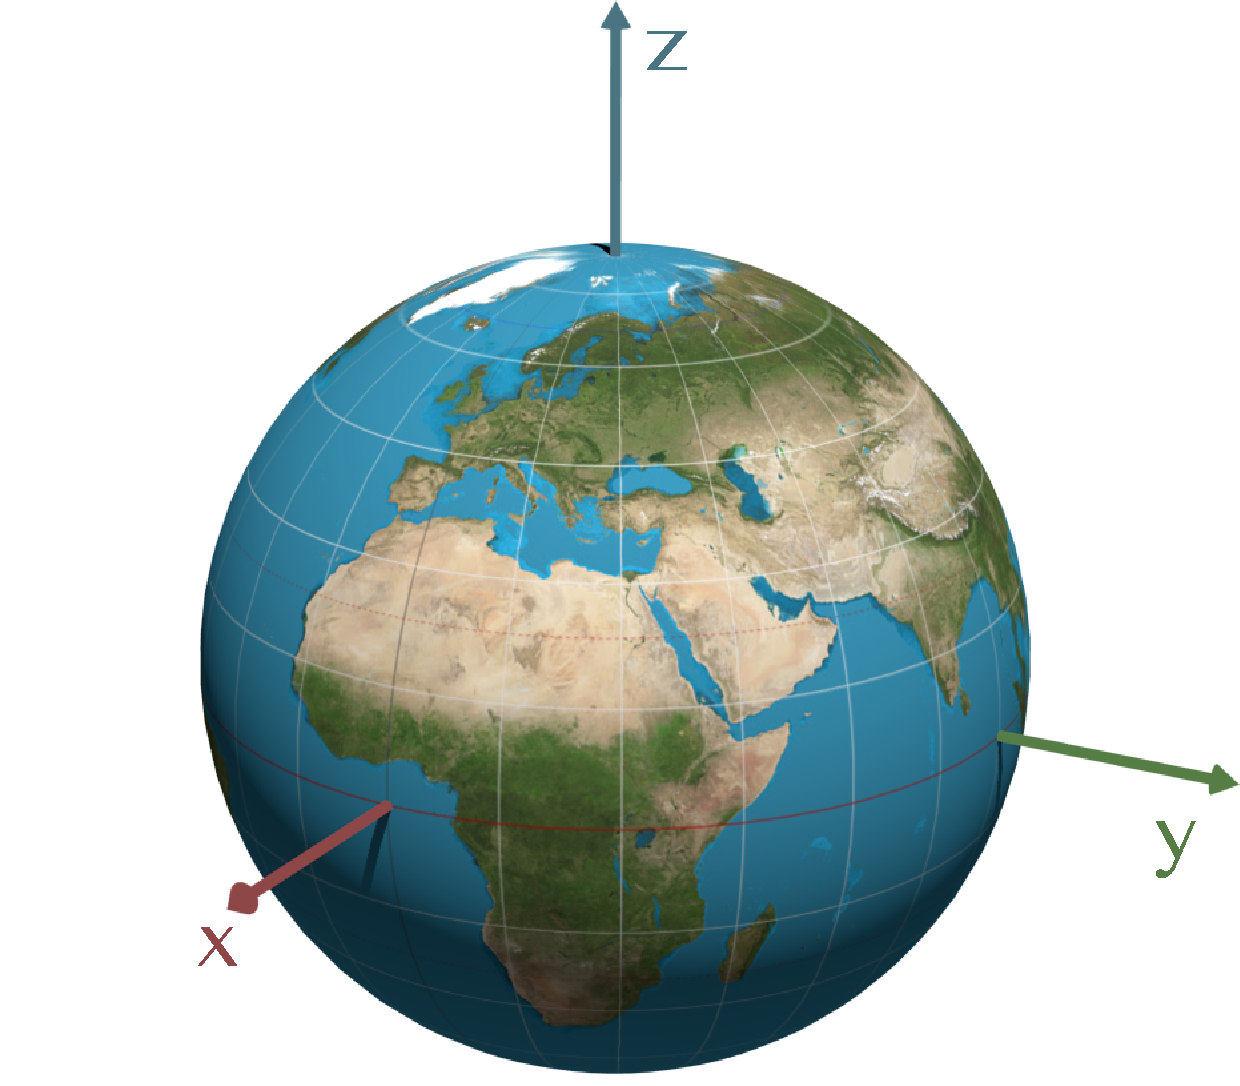
\includegraphics[scale=0.25]{figures/wgs84.pdf}
\caption{The WGS84 coordinate system and globe.}
\label{fig:wgs84}
\end{figure}

\subsection{Tesselating the Ellipsoid}

Triangle models are still the most common way of modeling renderable objects in 3D graphics softwares, even though other rendering techniques such as volumetric ray casting also is possible for terrain rendering (src).

A triangle mesh, or more generally a polygon mesh, is defined by a limited number of surface elements. This means that ellipsoids need to be approximated by some sort of tessellation or subdivision surface when modeled as a polygon mesh. There are several techniques for tessellating an ellipsoid. Some of them are covered in this section.

\subsubsection{Geographic Grid Tessellation}
\label{sec:geogrid}
Tessellating the ellipsoid using a geographic grid is a very straightforward approach. Ellipsoid vertex positions can be calculated using a transform from geographic coordinates to cartesian model space coordinates \cite[p. 25]{cozzi11}. Figure \ref{fig:tesselation_geo} shows three geographic grid tessellations of ellipsoids with constant number of latitudinal segments of 4, 8 and 16 respectively.

A common issue with geographic grids is something referred to as polar pinching. At both of the poles, segments will be pinched to one point which leads to an increasing amount of segments per area. This in turn results in oversampling in textures as well as possible visual artefacts in shading due to the very thin quads at the poles as well as possible performance penalties for highly tessellated globes.

\begin{figure}
    \centering
    \begin{subfigure}[b]{0.2\textwidth}
        \includegraphics[width=\textwidth]{figures/tessellation/tessellation_geo1.png}
    \end{subfigure}
    ~ %add desired spacing between images, e. g. ~, \quad, \qquad, \hfill etc. 
      %(or a blank line to force the subfigure onto a new line)
    \begin{subfigure}[b]{0.2\textwidth}
        \includegraphics[width=\textwidth]{figures/tessellation/tessellation_geo2.png}
    \end{subfigure}
    ~ %add desired spacing between images, e. g. ~, \quad, \qquad, \hfill etc. 
    %(or a blank line to force the subfigure onto a new line)
    \begin{subfigure}[b]{0.2\textwidth}
        \includegraphics[width=\textwidth]{figures/tessellation/tessellation_geo3.png}
    \end{subfigure}
    \caption{Geographic grid tesselation.}
    \label{fig:tesselation_geo}
\end{figure}

\subsubsection{Quadrilateralized Spherical Cube Tessellation}
 
Another common tessellation method for spheres which can be generalized to ellipsoids is the quadrilateralized spherical cube tessellation. The standard approach is to subdivide a cube centered in the origin and then normalize the coordinates of all vertices to map them on a sphere. There are also other more complicated schemes designed to work with specific map projections \cite{dimi15}.

To model an ellipsoid from a sphere, the vertices can be linearly transformed with a scaling in the $x$, $y$, and $z$ directions individually. Figure \ref{fig:tesselation_cube} shows a tessellated spherical cube of four different detail levels.

\begin{figure}
    \centering
    \begin{subfigure}[b]{0.2\textwidth}
        \includegraphics[width=\textwidth]{figures/tessellation/tessellation_cube1.png}
    \end{subfigure}
    ~ %add desired spacing between images, e. g. ~, \quad, \qquad, \hfill etc. 
      %(or a blank line to force the subfigure onto a new line)
    \begin{subfigure}[b]{0.2\textwidth}
        \includegraphics[width=\textwidth]{figures/tessellation/tessellation_cube2.png}
    \end{subfigure}
    ~ %add desired spacing between images, e. g. ~, \quad, \qquad, \hfill etc. 
    %(or a blank line to force the subfigure onto a new line)
    \begin{subfigure}[b]{0.2\textwidth}
        \includegraphics[width=\textwidth]{figures/tessellation/tessellation_cube3.png}
    \end{subfigure}
    ~ %add desired spacing between images, e. g. ~, \quad, \qquad, \hfill etc. 
    %(or a blank line to force the subfigure onto a new line)
    \begin{subfigure}[b]{0.2\textwidth}
        \includegraphics[width=\textwidth]{figures/tessellation/tessellation_cube4.png}
    \end{subfigure}
    \caption{Quadrilateralized spherical cube tessellation.}
    \label{fig:tesselation_cube}
\end{figure}

\subsubsection{Hierarchical Triangular Mesh}

The hierarchical triangular mesh (HTM) is a method of modeling the sky dome as a sphere proposed by astronomers in the Sloan Digital Sky Survey \cite{htm}. Instead of uniformly dividing cube faces, an alternative option is to subdivide a normalized octahedron by, in each subdivision step, split every triangle into four new triangles, see figure \ref{fig:tesselation_htm}. An ellipsoid can be created from the sphere by normalizing the coordinates and linearly rescaling them the same way that can be done for the spherical cube tessellation.

\begin{figure}
    \centering
    \begin{subfigure}[b]{0.2\textwidth}
        \includegraphics[width=\textwidth]{figures/tessellation/tessellation_htm1.png}
    \end{subfigure}
    ~ %add desired spacing between images, e. g. ~, \quad, \qquad, \hfill etc. 
      %(or a blank line to force the subfigure onto a new line)
    \begin{subfigure}[b]{0.2\textwidth}
        \includegraphics[width=\textwidth]{figures/tessellation/tessellation_htm2.png}
    \end{subfigure}
    ~ %add desired spacing between images, e. g. ~, \quad, \qquad, \hfill etc. 
    %(or a blank line to force the subfigure onto a new line)
    \begin{subfigure}[b]{0.2\textwidth}
        \includegraphics[width=\textwidth]{figures/tessellation/tessellation_htm3.png}
    \end{subfigure}
    ~ %add desired spacing between images, e. g. ~, \quad, \qquad, \hfill etc. 
    %(or a blank line to force the subfigure onto a new line)
    \begin{subfigure}[b]{0.2\textwidth}
        \includegraphics[width=\textwidth]{figures/tessellation/tessellation_htm4.png}
    \end{subfigure}
    \caption{Hierarchical triangular mesh tesselation.}
    \label{fig:tesselation_htm}
\end{figure}

\subsubsection{Hierarchical Equal Area IsoLatitude Pixelation}

Hierarchical Equal Area IsoLatitude Pixelation (HEALPix) is spherical tessellation scheme with corresponding map projection. The base level of the tessellation is built up of twelve quads, similar to a rhombic dodecahedron, which each can be subdivided further. The tessellation in figure \ref{fig:tesselation_healpix} shows how the vertices in the HEALPix tessellation leads to curvilinear quads.

\begin{figure}
    \centering
    \begin{subfigure}[b]{0.2\textwidth}
        \includegraphics[width=\textwidth]{figures/tessellation/tessellation_healpix1.png}
    \end{subfigure}
    ~ %add desired spacing between images, e. g. ~, \quad, \qquad, \hfill etc. 
      %(or a blank line to force the subfigure onto a new line)
    \begin{subfigure}[b]{0.2\textwidth}
        \includegraphics[width=\textwidth]{figures/tessellation/tessellation_healpix2.png}
    \end{subfigure}
    ~ %add desired spacing between images, e. g. ~, \quad, \qquad, \hfill etc. 
    %(or a blank line to force the subfigure onto a new line)
    \begin{subfigure}[b]{0.2\textwidth}
        \includegraphics[width=\textwidth]{figures/tessellation/tessellation_healpix3.png}
    \end{subfigure}
    \caption{HEALPix tesselation.}
    \label{fig:tesselation_healpix}
\end{figure}

\subsubsection{Geographic Grid Tessellation With Polar Caps}

In their description of the ellipsoidal clipmaps method, Dimitrijevi\'{c} and Ran\v{c}i\'{c} introduces polar caps to avoid polar issues related to geographic grids \cite{dimi15}. The polar caps are simply used as a replacement of the problematic, oversampled regions around the poles. The caps can be modelled as grids projected onto the ellipsoid surface in their own georeferenced coordinate systems. One obvious issue with polar caps is the edge problem that occurs due to the fact that the caps are defined as separate meshes with vertices that do not coincide with the geographic vertices of the equatorial region, see figure caps. Dimitrijevi\'{c} and Ran\v{c}i\'{c} solves the issue by using a type of edge blending between the equatorial and polar segments \cite{dimi15}. Figure \ref{fig:tesselation_caps} shows a sphere tessellated with one equatorial region and two polar regions.

\begin{figure}
    \centering
    \begin{subfigure}[b]{0.2\textwidth}
        \includegraphics[width=\textwidth]{figures/tessellation/tessellation_caps_proj1.png}
    \end{subfigure}
    ~ %add desired spacing between images, e. g. ~, \quad, \qquad, \hfill etc. 
      %(or a blank line to force the subfigure onto a new line)
    \begin{subfigure}[b]{0.2\textwidth}
        \includegraphics[width=\textwidth]{figures/tessellation/tessellation_caps_proj2.png}
    \end{subfigure}
    ~ %add desired spacing between images, e. g. ~, \quad, \qquad, \hfill etc. 
    %(or a blank line to force the subfigure onto a new line)
    \begin{subfigure}[b]{0.2\textwidth}
        \includegraphics[width=\textwidth]{figures/tessellation/tessellation_caps_proj3.png}
    \end{subfigure}
    \caption{Geographic tessellation of an ellipsoid with polar caps.}
    \label{fig:tesselation_caps}
\end{figure}

\subsection{2D Parameterisation for Map Projections}

A map projection $P$ defines a transformation from cartesian model space coordinates to georeferenced (projected) coordinates, as in equation \ref{eq:proj}. The inverse projection $P^{-1}$ is used to find positions on the globe surface in model space given georeferenced coordinates as in equation \ref{eq:invproj}.

\begin{equation}
\label{eq:proj}
\begin{pmatrix} s  \\ t  \end{pmatrix}_{ georeferenced }=\vec { P } (x,y,z),
\end{equation}

\begin{equation}
\label{eq:invproj}
\begin{pmatrix} x \\ y \\ z \end{pmatrix}_{ modelspace }=\vec { P }^{-1} (s ,t ),
\end{equation}

Where $(x,y,z)^T$ is the cartesian coordinates of a point on the ellipsoid surface. The parameters $s$ and $t$ are georeferenced coordinates defining all positions on the globe. The georeferenced coordinates can have different definition range depending on which projection is used.

The globally positive gaussian curvature of any ellipsoid makes it impossible to unproject it on a flat 2D surface without any distortions. Different projections are used for different purposes. Equal-area projections preserve the size of a projected area as $\partial s \partial t / \partial s_0 \partial t_0 = 1$, while conformal projections preserve the shape of projected objects as $\partial s / \partial t = 1$; $s_0$ and $t_0$ are coordinates at the center of the projection with no distortion. No global projection can be both area-preserving and conformal \cite{dimi15}.

There are several possibilities for defining a coordinate transform for map projections. A common approach is to project the ellipsoid onto another shape that allows for being flattened out without distortion, such as a cube, a cylinder or a plane. These types of shapes are known as developable shapes and have zero gaussian curvature.

The choice of map projection is tied together with the choice of ellipsoid tessellation. This is because the map often needs to be tiled up when rendering. Each tile has its local texture coordinate system which need to have a simple transform from the georeferenced coordinate system for texture sampling. If the tiles can be affinely transformed to the geo referenced coordinate system, texture sampling can be done on the fly; otherwise the geo referenced coordinates need to be reprojected which may be computationally heavy or impossible for real time applications.

The European Petroleum Survey Group (EPSG) has defined several standards for map projections of the Earth. Many of these are mentioned when discussing the different projections.

\subsubsection{Geographic Projections}

Geographic projections are widely used standards for parameterization of ellipsoids. The ellipsoid is projected onto a cylinder which is then unrolled to form the 2D plane of the projected coordinates.

Geographic coordinates are defined with a latitude $\phi$ and a longitude $\theta$ and works together with geographic tessellations of ellipsoids. A common issue with geographic projections is oversampling around the poles, as mentioned in section \ref{sec:geogrid}. At the poles, all longitudes will always map onto one point and the distortion increases with the absolute value of the latitude. Figure \ref{fig:proj_equi} shows an unprojected geographic map and how it wraps around the globe.

\begin{figure}[htbp]
    \centering
    \begin{subfigure}[bt]{0.4\textwidth}
        \includegraphics[width=\textwidth]{figures/developable_projected/equirectangular.png}
    \end{subfigure}
    \qquad
    \begin{subfigure}[bt]{0.15\textwidth}
        \includegraphics[width=\textwidth]{figures/map_projection/projection_geo.png}
    \end{subfigure}
    \caption{Geographic map projection.}
    \label{fig:proj_equi}
\end{figure}

\paragraph{Geocentric projection}
The simplest geographic parameterization uses geocentric coordinates. Here the latitude and longitude are defined as the angle between a vector from the origin to a point on the ellipsoid surface, and the $xy-$ and $xz-$planes respectively.

\paragraph{Geodetic projection}
The equirectangular cylindrical projection, using geodetic coordinates, is another variety of the geographic coordinate systems where the distance differential along the latitude $\partial \phi$ maps linearly to the latitude differential of the projected coordinates of the map.

Figure \ref{fig:geodetic} shows the difference between geocentric latitudes, $\phi_c$ and geodetic latitudes, $\phi_d$ for a point $\vec{p}$ on the surface of an ellipsoid. The figure also shows the difference between geocentric and geodetic surface normals, $\hat{n_c}$ and $\hat{n_d}$, respectively. 

\begin{figure}[htbp]
\centering
\begin{picture}(130,130)
    \put(0,0){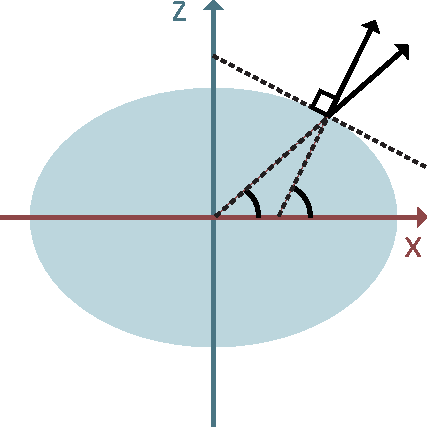
\includegraphics[width=0.35\textwidth]{figures/geodetic_geocentric.pdf}}
    \put(112,97){$\vec{p}$}
    \put(130,107){$\hat{n}_c$}
    \put(100, 130){$\hat{n}_d$}
    \put(100, 75){$\phi_d$}
    \put(82, 75){$\phi_c$}
    \label{fig:proj_equirectangular}
\end{picture}
\caption{Difference between geocentric and geodetic latitudes.}
\label{fig:geodetic}
\end{figure}

In the case of perfect spheres, geocentric and geodetic projections of any point will yield the same result.

Geodetic coordinates are among the most commonly used geo referenced coordinate systems when mapping ellipsoids to two dimensions. Latitudinal distances are preserved after the coordinate transform. This is important for a map projection standard that can be used for both spheres and for ellipsoids to avoid distortions that will appear if the map is defined for a specific ellipsoid and then projected on a slightly different one.

Equirectangular projections does not require specific ellipsoids to avoid distorsions on the mapped globe. The result of the wide usage is that many map providers choose to provide 2D maps defined in this coordinate system.

Cozzi and Ring describes the transform from geodetic coordinates in the ellipsoid class \cite[p. 25]{cozzi11}. For the Earth, the most commonly used geodetic coordinate space is defined in the EPSG:4326 standard where the WGS84 ellipsoid is used.

\subsubsection{Mercator Projection}

The mercator projection is a cylindrical projection widely used for presenting global maps in unwrapped form. The mercator projection preserves the horizontal to vertical ratio for small objects on the map. Hence, the mercator is a conformal projection in contrast to the geocentric and geodetic projections, which results in a non unit value in the ratio between the longitudinal and latitudinal differentials, see figure \ref{fig:mercator}.

\begin{figure}[htbp]
    \centering
    \begin{subfigure}[bt]{0.3\textwidth}
        \includegraphics[width=\textwidth]{figures/central_park_equirectangular.png}
	\caption{The equirectangular projection is not conformal.}
    \end{subfigure}
    \qquad
    \begin{subfigure}[bt]{0.3\textwidth}
        \includegraphics[width=\textwidth]{figures/central_park_mercator.png}
        \caption{The mercator projection is conformal and preserves aspect ratio.}
    \end{subfigure}
    \caption{Unwrapped equirectangular and mercator projections.}
    \label{fig:mercator}
\end{figure}

The mercator projection compensates for the longitudinal distortion by introducing a latitudinal distortion as well. Due to the polar singularities which lead to infinite latitudes at the poles when $\phi_d = \pm 90$, the domain of definition for the latitudes need to be constrained in mercator projection, see figure mercator.

\begin{figure}[htbp]
    \centering
    \begin{subfigure}[bt]{0.4\textwidth}
        \includegraphics[width=\textwidth]{figures/developable_projected/mercator.png}
    \end{subfigure}
    \qquad
    \begin{subfigure}[bt]{0.15\textwidth}
        \includegraphics[width=\textwidth]{figures/map_projection/projection_mercator.png}
    \end{subfigure}
    \caption{Mercator projection.}
    \label{fig:proj_mercator}
\end{figure}

The EPSG:3857 standard for mercator projection of the Earth, also known as web mercator, constrains the domain to $\phi \in [-85.06, 85.06]$. The standard uses a different projection that does not diverge at the polar regions. Web mercator is used by most online web map applications including Google Maps, Bing Maps, OpenStreetMap, Mapquest, Esri and Mapbox \cite{battersby14}.

\subsubsection{Cube Map}

Cube maps lack the polar singularities apparent in geographic parameterizations. The parameterized coordinates are often discretized to the six sides of the cube, but they can also map directly to a global representation of an unwrapped cube, see figure \ref{fig:proj_cube}.

\begin{figure}[htbp]
    \centering
    \begin{subfigure}[bt]{0.4\textwidth}
        \includegraphics[width=\textwidth]{figures/developable_projected/cube_map.png}
    \end{subfigure}
    \qquad
    \begin{subfigure}[bt]{0.15\textwidth}
        \includegraphics[width=\textwidth]{figures/map_projection/projection_cube.png}
    \end{subfigure}
    \caption{Cube map projection.}
    \label{fig:proj_cube}
\end{figure}

Due to the traditions of map projections this is not a common format used for map services so reprojection from a more common format is often required.

There are different cube map projections with different amount of area- and aspect distortions. Dimitrijevi\'{c} and Ran\v{c}i\'{c} mention and compares spherical cube, adjusted spherical cube, Outerra spherical cube and quadrilateralized spherical cube \cite{dimi15}.

\subsubsection{Tessellated Octahedral Adaptive Subdivision Transform}

The Tessellated Octahedral Adaptive Subdivision Transform (TOAST) map format used in the globe browsing of Microsoft's World Wide Telescope works together with the HTM tessellation \cite{toast}. Each triangular segment of the TOAST map maps linearly to a triangle of a sphere that is tessellated as an octahedron and subdivided to form a sphere, see figure \ref{fig:proj_toast}.

\begin{figure}[htbp]
    \centering
    \begin{subfigure}[bt]{0.3\textwidth}
        \includegraphics[width=\textwidth]{figures/developable_projected/toast.png}
    \end{subfigure}
    \qquad
    \begin{subfigure}[bt]{0.2\textwidth}
        \includegraphics[width=\textwidth]{figures/map_projection/projection_toast.png}
    \end{subfigure}
    \caption{TOAST map projection.}
    \label{fig:proj_toast}
\end{figure}

The TOAST format is just as the cube maps not a very well supported format for map providers and harder to use together with some of the most common level of detail approaches due to the fact that most of them are optimized for rectangular and not triangular map tiles.

\subsubsection{Hierarchical Equal Area IsoLatitude Pixelation}

The map projection that is used for the HEALPix tessellation is equal-area as the name suggests. Figure \ref{fig:proj_healpix} shows how the map wraps onto the sphere. The positive aspect about HEALPix compared to the TOAST format is that the map is tiled into quads and not triangles which means that it is better suitable for the chunked lod \cite{cozzi11} algorithm. The map format is used by the Sloan Digital Sky Survey for mapping the cosmic microwave background radiation but is otherwise an uncommon format when it comes to map services. That means that the maps need to be reprojected from the more common formats for wider support.

\begin{figure}[htbp]
    \centering
    \begin{subfigure}[bt]{0.5\textwidth}
        \includegraphics[width=\textwidth]{figures/developable_projected/healpix.png}
    \end{subfigure}
    \qquad
    \begin{subfigure}[bt]{0.2\textwidth}
        \includegraphics[width=\textwidth]{figures/map_projection/projection_healpix.png}
    \end{subfigure}
    \caption{HEALPix map projection.}
    \label{fig:proj_healpix}
\end{figure}

\subsubsection{Polar Projections}

For parameterization of limited parts of the globe, such as the isolated poles, there are different projections to consider. Most common are different types of azimuthal projections. These projections are defined by projecting all points of the map through a common intersection point and onto a flat surface. The Gnomonic projection maps all great circle segments (geodesics) to straight lines by having the common intersection point in the center of the globe.

Stereographic projections are defined when the common intersection point is positioned on the surface of the globe on the opposite side of the pole to project. Polar stereographic projections are used to parameterize the surface of the poles of the Earth. The standards EPSG:3413 and EPSG:3031 define the stereographic projections for the North Pole and the South Pole respectively.

Dimitrijevi\'{c} and Ran\v{c}i\'{c} uses another polar coordinate system to reproject from geodetic coordinates in runtime. The transformation is a rotation of 90 degrees around the global $x-$axis so that the resulting parametric coordinates of the pole are given in their own geographic space with the main meridian as equator. This projection is also known as a Cassini projection and it can be both defined for spheres as well as generalized to ellipsoids. Polar projections are shown in figure \ref{fig:proj_polar}.

\begin{figure}[htbp]
    \centering
    \begin{subfigure}[b]{0.3\textwidth}
        \includegraphics[width=\textwidth]{figures/map_projection/projection_cassini.png}
    	\caption{Cassini}
    \end{subfigure}
    ~
    \begin{subfigure}[b]{0.3\textwidth}
        \includegraphics[width=\textwidth]{figures/map_projection/projection_gnomonic.png}
        \caption{Gnomonic}
    \end{subfigure}
    ~
    \begin{subfigure}[b]{0.3\textwidth}
        \includegraphics[width=\textwidth]{figures/map_projection/projection_stereographic.png}
    	\caption{Stereographic}
    \end{subfigure}
    \caption{Polar map projections.}
    \label{fig:proj_polar}
\end{figure}


\subsection{Dynamic Level of Detail}
Dynamic level of detail (LOD) is an important part in handling the extensive amount of data used in an out of core rendering software. The goal is to maximize the visual information on screen while minimizing the workload. In their book Rendering virtual 3D globes, Cozzi and Ring describes LOD rendering algorithms by three typical steps. \cite[p. 367]{cozzi11}

\begin{enumerate}
    \item Generation - Create versions at different level of detail of a model
    \item Selection - Choose a version based on some criteria or error metric (e.g., distance to object or the projected area it occupies on the screen)
    \item Switching - Transitions from one version to another in order to avoid noticing of the change in LOD known as popping artifacts.
\end{enumerate}

There are different types of LOD approaches for terrain rendering, and a suitable approach should be chosen based on characteristics of the terrain. Terrains can for example be restricted to being represented as height maps - a characteristic that can be exploited by the rendering algorithm. Cozzi and Ring describe the following three categories of LOD approaches: Discrete Level of Detail, Continuous Level of Detail and Hierarchical Level of Detail \cite[p. 368-371]{cozzi11}.

\subsubsection{Discrete Level of Detail}
In the Discrete Level Of Detail (DLOD) approach, multiple different representations of the terrain are created at different resolutions. DLOD is arguably the most simple LOD algorithm. It works not only for digital terrain models, but for arbitrary meshes. The set of terrain representations can either be predefined or generated using mesh simplification algorithms.

\begin{figure}[htbp]
    \centering
    \begin{subfigure}[bt]{0.9\textwidth}
        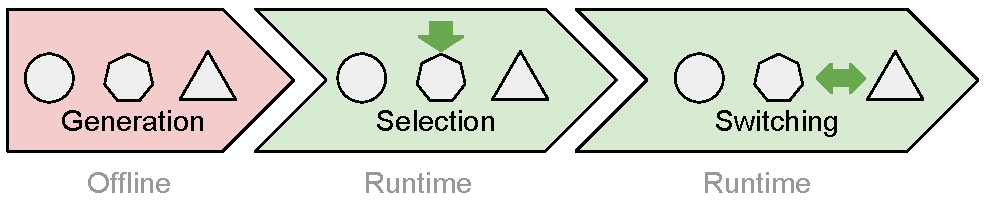
\includegraphics[width=\textwidth]{figures/lod/lod_overview.pdf}
    \end{subfigure}
    \caption{DLOD. Generate offline, select and switch at runtime.}
    \label{fig:lod}
\end{figure}

\begin{figure}
    \centering
    \begin{subfigure}[b]{0.2\textwidth}
        \includegraphics[width=\textwidth]{figures/lod/decimation1.png}
    \end{subfigure}
    ~ %add desired spacing between images, e. g. ~, \quad, \qquad, \hfill etc. 
      %(or a blank line to force the subfigure onto a new line)
    \begin{subfigure}[b]{0.2\textwidth}
        \includegraphics[width=\textwidth]{figures/lod/decimation2.png}
    \end{subfigure}
    ~ %add desired spacing between images, e. g. ~, \quad, \qquad, \hfill etc. 
    %(or a blank line to force the subfigure onto a new line)
    \begin{subfigure}[b]{0.2\textwidth}
        \includegraphics[width=\textwidth]{figures/lod/decimation3.png}
    \end{subfigure}
    \caption{A range of predefined meshes with decreasing resolution}
    \label{fig:dlod}
\end{figure}

At run time, the main objective is to select one (or generate) a suitable representation. This approach does not provide any means of dealing with large scale datasets, which makes it unsuitable for globe rendering (ref virtual globes).

\subsubsection{Continuous Level of Detail}
The continuous LOD (CLOD) approach represents a model in a way that allows the resolution to be selected arbitrary. This is usually implemented by a base mesh combined with a sequence of operations that successively changes the level of detail of the model. Two typical such operations are ``edge collapse'' (removes two triangles from the mesh) and its inverse, ``vertex split'' (adds two triangles to the mesh). 

\begin{figure}
    \centering
    \begin{subfigure}[b]{0.2\textwidth}
        \includegraphics[width=\textwidth]{figures/lod/vertex_split1.png}
    \end{subfigure}
    ~ %add desired spacing between images, e. g. ~, \quad, \qquad, \hfill etc. 
      %(or a blank line to force the subfigure onto a new line)
    \begin{subfigure}[b]{0.2\textwidth}
        \includegraphics[width=\textwidth]{figures/lod/vertex_split2.png}
    \end{subfigure}
    \caption{Edge collapse in continous LOD}
    \label{fig:clod}
\end{figure}

According to Cozzi and Ring \cite[p. 368]{cozzi11} CLOD has previously been the most popular approach for rendering terrain at interactive rates, with implementations such as Real-time Optimally Adaptive Mesh (ROAM). The main reason CLOD algorithms are not widely employed these days is due to the increase in triangle throughput on modern GPUs, causing the CLOD operations done on the CPU in many cases to act as a bottleneck for the rendering time.

A special branch of CLOD worth mentioning is the so called infinite LOD. In this approach the terrain is represented by a mathematical function - an implicit surface. These functions can be defined by fractal algorithms and produce complex characteristics, or they can define simple geometric shapes such as spheres or ellipsoids. As every point on these types of surfaces are precisely defined, triangle meshes can be generated with no limit on the level of detail. This approach is not suitable for incorporating real world data, but it is used by terrain engines such as Outerra and Terragen to procedurally generate terrain at any desired level of detail \cite{outerraprocedural09}. 

\subsubsection{Hierarchical Level of Detail}
Hierarchical Level of Detail (HLOD) can be seen as a generalization of DLOD. HLOD algorithms operates on hierarchically arranged, predefined chunks of the full model. Each chunk is processed, stored and rendered separately. By doing this, HLOD approaches tackles the weaknesses of CLOD, essentially by doing the following.

\begin{enumerate}
    \item Reduce processing time on CPU: The only CPU task that HLOD algorithms has to deal with during runtime is to select a suitable subset of the predefined chunks for rendering. This is a relatively fast procedure in contrast to iteratively applying changes to the raw geometry, as done in CLOD.
    \item Reduce the data traffic to GPU: Data is uploaded to the GPU in larger batches but not very often, since the data is static and GPU caching can be done. With CLOD, the geometry data is updated on a per-frame basis, and can't be cached on the GPU. Being able to perform GPU caching allow HLOD to better minimize the traffic to the GPU.
\end{enumerate}

HLOD uses spatial hierarchical data structures such as quadtrees or octrees for storing the chunk data. The root node of the tree holds a full representation of the model at its lowest level of detail a one single chunk. At successive levels, the model is represented at a higher level of detail but divided up into several chunks. This concept is illustrated in figure hlod.

\begin{figure}[htbp]
    \centering
    \begin{subfigure}[bt]{0.4\textwidth}
        \includegraphics[width=\textwidth]{figures/lod/hlod_tmp.png}
    \end{subfigure}
    \caption{HLOD using a quadtree.}
    \label{fig:hlod}
\end{figure}

Generally, selecting all the chunks at a specific level in the tree yields a complete representation of the model. Furthermore, chunks may be selected from different levels for different parts of the model and still yield a full representation of the model. This allows for view dependent rendering of the model. Algorithm chunk selection describes pseudo code for recursively rendering the full model at view dependent level of detail.

\begin{algorithm}[htp]
  \SetKwFunction{RenderLOD}{}
  \SetKwProg{myalg}{RenderLOD}{}{}
  \myalg{\RenderLOD{Camera C, ChunkNode N}}{
  \eIf{ErrorMetric($C$, $N$) < threshold}{
        Render($N$, $C$)
    }{
        \For{$child$ \textbf{in} $children(N)$}{
            RenderLOD($child$, $C$)
        }
    }
  }{}
  \caption{Algorithm with procedure}
\end{algorithm} 


This example uses a depth first approach for rendering of chunks. Other common schemes for traversing the hierarchy are breadth first and inverse breadth first.

The algorithm traverses the tree and calculates an error metric at each node with respect to the current camera position. If the calculated error is larger than a certain threshold, the algorithm recursively repeats the procedure for all the chunk's children, which has higher level of detail. This general scheme can be used for rendering one-dimensional curves (using a binary tree structure), two-dimensional surfaces (using a quadtree) or volumes (using an octree).

Another key feature of HLOD as opposed to DLOD and CLOD is that it can naturally be integrated with out-of-core rendering, as chunks can be loaded into memory on-demand and thrown away when not needed.

\section{Large Scale Map Datasets}

Global maps with high level of detail can easily become too large to be stored and read locally on a single machine. A common way of storing large maps is by representing them using several overviews. An overview is a map representing the same geographical area as the original map but containing only one fourth as many pixels just like a lower level of a mip map texture. Figure \ref{fig:overview} shows how the size of the maps in raster coordinates decreases with the overview number.

\begin{figure}[htbp]
    \centering
    \begin{picture}(130,60)
        \put(0,0){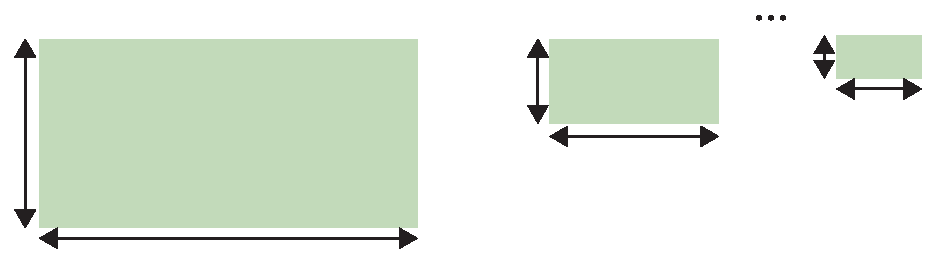
\includegraphics[width=0.5\textwidth]{figures/overview.pdf}}
    	\put(-50,50){Overview:}
    	\put(45,50){0}
    	\put(127,50){1}
    	\put(176,50){n}
    	\put(-5,25){$y$}
    	\put(45,-5){$x$}
	\put(100,35){$\frac{y}{2}$}
	\put(127,15){$\frac{x}{2}$}
	\put(155,37){$\frac{y}{2^n}$}
    	\put(176,25){$\frac{x}{2^n}$}

    	\label{fig:proj_equirectangular}
    \end{picture}
    \caption{The size of the map is decreasing exponentially with the overview.}
    \label{fig:overview}
\end{figure}

The physical disk space of large global map datasets is often measured in terabytes or even petabytes. In order to deal with such large datasets, web based services allow users to specify only parts of the map to download at a time. This is an important aspect in the out of core rendering required for globe visualization.

\subsection{Web Map Services}

To standardize web requests for map data, the Open GIS Consortium (OGS) specified a web map service interface \cite{wms06} and from that, specifications of several other map service interfaces have followed. The most common standards are Web Map Service (WMS), Tile Map Service (TMS) and Web Map Tile Service (WMTS). Some more specific examples of WMS-like services are WorldWind, VirtualEarth and AGS. The last three are not covered in this thesis.

\subsubsection{WMS}

The WMS interface produces maps as image files with well defined geographic and dimensional parameters. The image files can have different format and compression depending on the provider. A WMS server has the ability to dynamically produce map patches of arbitrary size which puts some load on the server side \cite{wms06}. The basic elements supported by all WMS providers are the \emph{GetCapabilities} and the \emph{GetMap} operations. \emph{GetCapabilities} gives information about the available maps on the server and their corresponding geo referenced metadata. The \emph{GetMap} operation returns the map or a part of the map as an image file.

The structure of a WMS request using HTTP GET is of the form \\ \texttt{http://host\lbrack:port\rbrack/path\lbrack?\{name\lbrack=value\rbrack\&\}} where the name and value pairs are defined for each operation by the standard \cite{wms06}. For example, setting the parameter \texttt{BBOX=-180,-90,180,90} specifies the size of the map in geo referenced coordinates while the parameters \texttt{WIDTH} and \texttt{HEIGHT} specifies the requested image in raster coordinates. All name and value pairs for the \emph{GetMap} request are defined under the reference \cite{wms06}.


\chapter{Implementation}
The virtual globe rendering system was implemented as a separate module, programmed in C++ for OpenSpace which, if desired, can be opted out when building the software in CMake. The implementation defines a namespace with all the necessary data structures, classes and functionality specifically related to globe rendering. The basic structure of a \class{Renderable Globe} with its necessary components is illustrated as a UML diagram in figure \ref{fig:renderableglobe}.

\begin{figure}[htbp]
    \centering
    \begin{subfigure}[bt]{0.8\textwidth}
        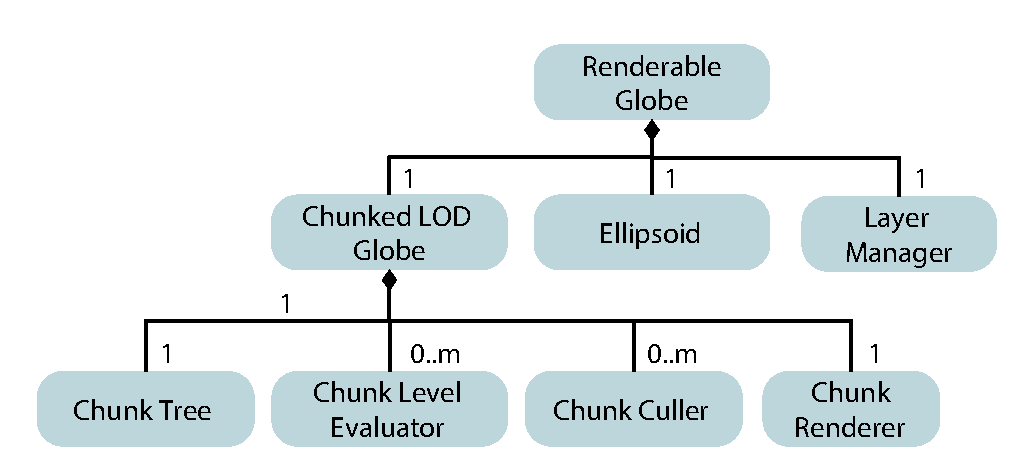
\includegraphics[width=\textwidth]{figures/implementation/renderable_globe.pdf}
    \end{subfigure}
    \caption{Overviewing class diagram of \class{Renderable Globe} and its related classes.}
    \label{fig:renderableglobe}
\end{figure}

The base of the globe renderer uses a modified version of Cozzi and Rings Chunked LOD algorithm. The globe is tessellated as an ellipsoid with a geometrical grid using geodetic map projection.

The full LOD rendering system required several components of different complexity to be implemented. All components will be described in detail in this chapter.

\section{Reference Ellipsoid}
The \class{Ellipsoid} class was implemented to handle all geographic related calculations.  These calculations include conversions between geodetic and cartesian coordinates and different kinds of projections onto the ellipsoid surface. These calculations are sped up by internal caching of a range of precalculated values. Cozzi and Ring provide a complete reference on the implementation \cite[p. 17]{cozzi11}.

The \class{Ellipsoid} uses several geographically related classes, which were used in multiple places within the implementation. These are:
\begin{enumerate}
	\item \class{Angle} - Handles angle related arithmetics, normalizations and unit abstractions (degrees and radians)
	\item \class{Geodetic2} - Represents a 2D geodetic coordinate (latitude, longitude)
	\item \class{Geodetic3} - Represents a 3D geodetic coordinate (latitude, longitude, altitude)
	\item \class{GeodeticPatch} - Represents a rectangular region in geodetic space
\end{enumerate}

\section{Chunked LOD}
The base of the chunked LOD algorithm revolves around the self updating chunk tree. The chunk tree is a data structure built up of \class{Chunk Node}s which have the ability to split or merge dynamically. Besides storing four \class{Chunk Node} children, each \class{Chunk Node} stores a \class{Chunk}.

\subsection{Chunks}
As opposed to the definition of chunks in the background section \ref{section:chunkedlodbacground}, this implementation of chunks is very lightweight - it does not store any texture or triangle mesh data. Instead, it stores the information needed to query texture tiles from local in-memory caches. In the implementation suggested by Cozzi and Ring, terrain triangle meshes are stored in each chunk. In the case of this implementation however, all terrain is rendered using height mapped vertex grids. Thus there is no need for each chunk to store their own vertex arrays. Instead they can simply share one single instance of a vertex grid within a whole chunk tree. This means that vertices need to be offset by height mapping on the GPU which makes it possibly to dynamically change height datasets that does not require pre processing before they can be used for rendering.

The most important part of the chunked LOD algorithm is the ability to dynamically select which chunks to split or merge. 

\subsection{Chunk Selection}
\label{section:chunkselection}
The chunk tree is automatically reshaped depending on the virtual camera. A chunk node splits, merges or remain the same depending on the chunk's error metric for the current LOD. Three different approaches for calculating the error metric were implemented. By letting the user dynamically adjust a LOD scale factor, performance can be weighted against detail level.

\subsubsection{By Distance}
By letting the error depend on the distance between the closest point on the chunk, and the camera $d$ as in Equation \ref{eq:loddistance}, the size of the chunks in screen space stays more or less constant.

\begin{equation}
	\label{eq:loddistance}
	e = l - log_2(\frac{s}{d}),
\end{equation}
where $e$ is the error, $l$ is the current level of the chunk, $s$ is a LOD scaling factor and $d$ is the distance between the closest point of the chunk and the camera. The closest point of the chunk can be either a corner or a point along one of the chunk edges. Using this distance as an error metric leads to bigger chunks farther from the camera where less detail is needed.


\subsubsection{By Projected Area}
Another error metric is the area that the chunk takes up on the screen. The bigger the area, the bigger the error. 

The error must not be dependent of the direction of the camera. This is because a chunk rendered on a multi screen display, such as a dome, should not have different errors between two or more screens which might lead to different levels and tearing between screens. Therefore the chunk is projected on a unit sphere and not a view plane which would lead to view direction dependent error metrics.

\begin{figure}[htbp]
    \centering
    \begin{subfigure}[bt]{0.5\textwidth}
        \includegraphics[width=\textwidth]{figures/implementation/chunklod/projectedarea.png}
    \end{subfigure}
    \caption{Triangle with the area 1/8 of the chunk projected onto a unit sphere}
    \label{fig:chunkprojarea}
\end{figure}

The projected area is a solid angle approximated by extracting three points on the chunk and projecting them on a unit sphere centered in the camera position. The three points define the closest of the four center triangles on the chunk, see Figure \ref{fig:chunkprojarea}. It is important that the triangle chosen for approximating the projected area can never have two vertices on the same upper or lower most edge. Such triangles (colored gray in Figure \ref{fig:chunkprojarea}) may have null areas at the poles, thus cannot be used to approxate the area of the full chunk.

The actual approximated solid angle is the projected triangle area multiplied by eight to accommodate a full chunk. This area is then subtracted by a constant value and scaled by a LOD scale factor to give similar LOD scaling as the distance dependent chunk selection.

\subsubsection{By Available Tile}
Splitting a chunk will not result in higher level of detail unless the corresponding higher level of detail tile data is also currently available for rendering. Therefore, the growth of the chunk tree can be limited by checking if there is any tile data there in the first place. This is useful in two scenarios:

\begin{enumerate}
\item Rendering of sparse map datasets which contain geographical regions where there are no data.
\item Rendering of map datasets which are queried from remote servers; there will always be some delay where the queried map data is not yet available.
\end{enumerate}

Being able to limit the chunk tree in these two scenarios, unnecessary chunk rendering calls can be avoided.

\subsection{Chunk Culling}
Given a chunk tree with chunks selected based on the camera position, each chunk can be tested using chunk cullers to determine if they are ``cullable'' and therefore can be set to invisible so that the chunk renderer will not bother in rendering them. The two implemented chunk cullers are the frustum culler and the horizon culler. They both rely on - and have access to - minimum and maximum values of the chunk's height maps. 

\subsubsection{Frustum Culling}
Frustum culling is implemented by first calculating a convex bounding polyhedron for the chunk to be tested. The bounding volume is calculated on the fly and takes into account any enabled height maps used to displace the vertices, making sure it fully encapsulates the displaced chunk vertices. The polyhedron is built up of eight vertices which are transformed to normalized device coordinates (NDC) using the view-projection matrix of the camera followed by perspective division. Once in NDC, an axis aligned bounding box (AABB) for the vertices is extracted. This AABB can then be tested against the screen bounds to determine if the chunk is outside the camera's field of view, and thus is cullable. This is illustrated in Figure \ref{fig:frustumculling}.

\begin{figure}[htbp]
    \centering
    \begin{subfigure}[bt]{1.0\textwidth}
        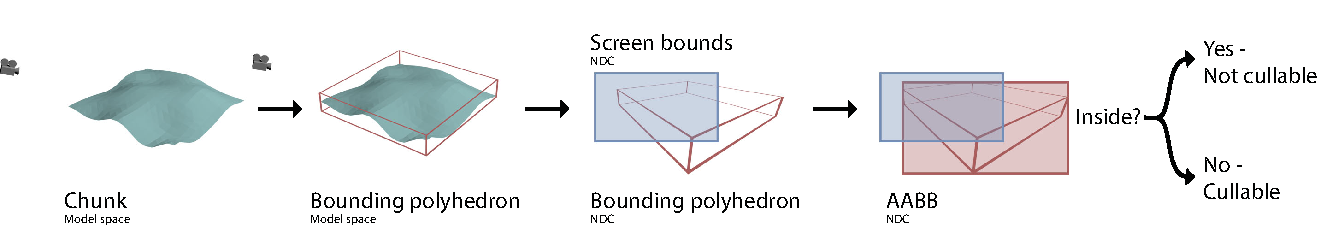
\includegraphics[width=\textwidth]{figures/implementation/chunklod/frustumculling.pdf}
    \end{subfigure}
    \caption{Frustum culling algorithm. This chunk cannot be frustum culled.}
    \label{fig:frustumculling}
\end{figure}

\subsubsection{Horizon Culling}
Given an object in position $\vec{p}$ with a bounding radius $r$ on the surface of the globe, it can be determined if it is completely behind the globe's horizon or not. The calculations are simplified by approximating the globe as a sphere using the minimum radius $r_g$ of its ellipsoid. Using the minimum radius and not a bigger number ensures that false occluding (chunks marked as invisible actually being visible) is not possible \cite[p. 393]{cozzi11}. The minimum allowed distance $l$ to the object can be calculated as the distance to the horizon $l_h$ added to the minimum allowed distance to the object from the horizon $l_m$. See figure \ref{fig:horizonculling}. Once the minimum allowed distance is calculated it can be compared to the actual distance to the object to determine if it is cullable or not.

\begin{figure}[htbp]
    \centering
    \begin{picture}(130,130)
        \put(0,0){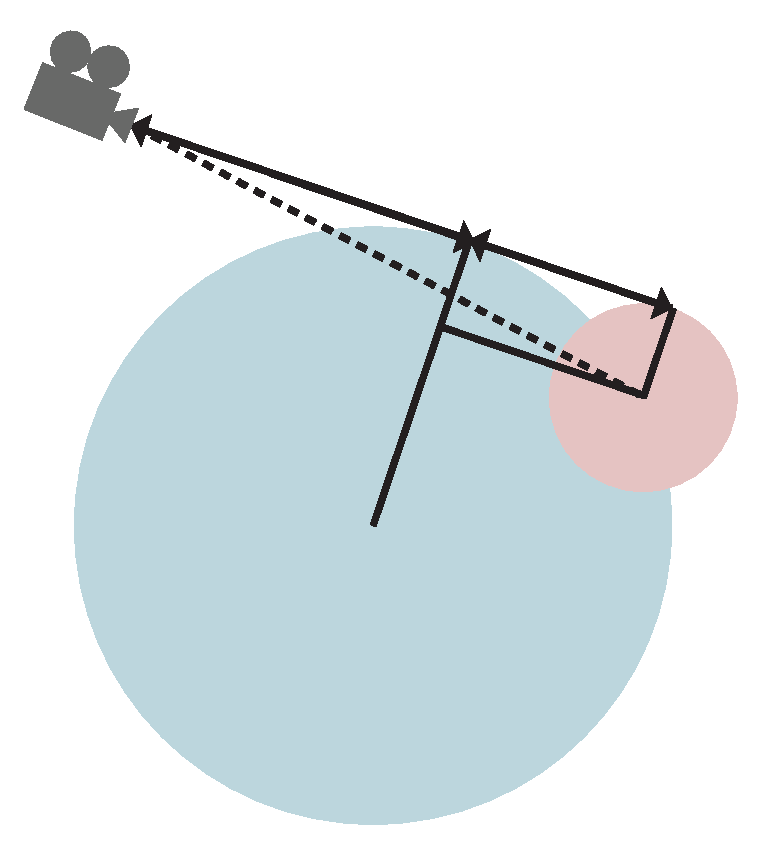
\includegraphics[width=0.4\textwidth]{figures/implementation/chunklod/horizonculling.pdf}}
        \put(60,145){$l_h$}
        \put(115,125){$l_m$}
        \put(135,95){$r$}
        \put(70,95){$r_g$}
        \put(130,80){$\vec{p}$}
        
    \end{picture}
    \caption{Horizon culling.}
    \label{fig:horizonculling}
\end{figure}

When culling chunks, the closest position on the chunk is used as the position $\vec{p}$ and the bounding height value as $r$.

\section{Reading and Tiling Image Data}
Fetching the right texture and preparing it for rendering onto chunks is a fairly complicated process. Before digging into the details of this process, there are three concepts that need to be established, as they will be referred to throughout the description of the texture pipeline. These are:

\begin{enumerate}
	\item \textbf{\class{Tile Index}} - A tuple of three integers $(level, x, y)$ indexing a specific map region on the globe.
	\item \textbf{\class{Raw Tile}} - A texture carved out to fit the geographical region of a specific chunk, along with meta data. Each \class{Raw Tile} is associated with a \class{Tile Index}. They can be instantiated concurrently.
	\item \textbf{\class{Tile}} - Like a \class{Raw Tile}, but the texture data is uploaded to the GPU and ready to use for rendering (unless it has a status not equal to ``OK''). As opposed to \class{Raw Tiles}, tiles rely on an OpenGL context and must therefore be initialized on the rendering thread.
\end{enumerate}

All chunk height and texture data are represented using \class{Tiles}. \class{Tiles} are created on the client side (i.e. in OpenSpace) on the fly when they are needed. As the pixel data may need to be read from disk or even requested from remote servers, the whole tile preparation pipeline was implemented to be executed on separate threads in order to avoid blocking of the rendering thread with image data reads. 

During the iterative process of developing the texture tile pipeline, three layers of abstraction were introduced in order to deal with the fairly high complexity. These are listed in Table \ref{table:tilepipeline}.

\begin{center}
  \begin{table}
  \caption[]{Abstraction layers used in the texture data pipeline.}
    \label{table:tilepipeline}
  \resizebox{\textwidth}{!}{\begin{tabular}{| c | c | c | c |}
    \hline
     Layer & \textbf{Component} 	& \textbf{Responsibility} & \textbf{Input --> Output} \\ \hline 
    3 & \class{Async Tile Dataset} 	& Async \class{Raw Tile} fetching  & \class{TileIndex} --> \class{Raw Tile} \\ \hline
    2 & \class{Tile Dataset}        & Tiling, georeferencing,  & \class{TileIndex} --> \class{Raw Tile} \\ 
     &         & preprocessing &  \\ \hline
    1 & GDAL         		& Image formats, I/O Operations, & pixel region --> pixel data \\
     &          		& georeferencing &  \\
    \hline
  \end{tabular}}
  \end{table}
\end{center}

The subsequent sections of this chapter will cover each abstraction layer in more detail, starting from the bottom and going up the stack.

\subsection{GDAL}
Geospatial Data Abstraction Library (GDAL) is an open source library providing a uniform interface for reading, manipulating and writing geospatial data in the form of raster and vector data models \cite{gdal}. GDAL is used as an abstraction layer between all the map formats and the representation of tile datasets. It provides an interface allowing client code to specify pixel regions within a dataset to read from, independent of the underlying image format. GDAL can also be used for disk based caching of data from remote servers. Reading pixel data using the GDAL RasterIO interface requires a set of parameters listed below and illustrated in Figure \ref{fig:gdalio}:

\begin{enumerate}
	\item A map overview to read pixel data from (if the dataset has overviews).
	\item A pixel region within that map overview to read pixels from.
	\item The raster band(s) (e.g., color channels) to read.
	\item A pointer to sufficient user allocated memory where GDAL can write the output of the read operation.
	\item The pixel region to write the output pixel data. The size of the pixel data to be written may differ from the pixel region to read from, in which case GDAL will resample and interpolate the pixel data automatically.
	\item The layout (i.e., pixel spacing, raster band spacing and line spacing).
	\item The data type to retrieve the pixel data in.
\end{enumerate}

\begin{figure}[htbp]
    \centering
    \begin{subfigure}[bt]{1.0\textwidth}
        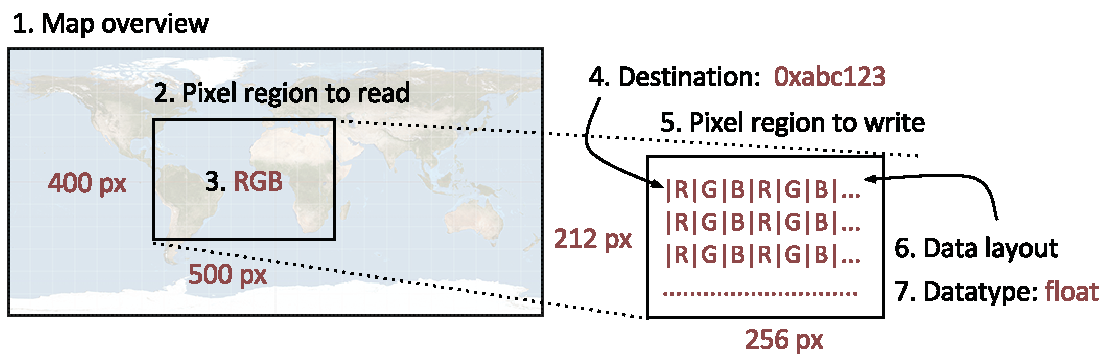
\includegraphics[width=\textwidth]{figures/implementation/pipeline/gdalio.pdf}
    \end{subfigure}
    \caption{The required GDAL raster IO parameters.}
    \label{fig:gdalio}
\end{figure}

With the given input parameters shown in Figure \ref{fig:gdalio}, the resulting output would be the pixel data of the requested image region written with the pixel layout parameters to the provided memory block. The output is illustrated in Figure \ref{fig:gdalioresult}.

\begin{figure}[htbp]
    \centering
    \begin{subfigure}[bt]{0.5\textwidth}
        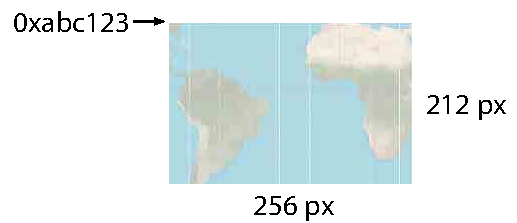
\includegraphics[width=\textwidth]{figures/implementation/pipeline/gdalioresult.pdf}
    \end{subfigure}
    \caption{Result of GDAL raster IO}
    \label{fig:gdalioresult}
\end{figure}

Using the RasterIO interface on an open GDAL dataset, the notion of image format is completely abstracted away. This is a great advantage which also allows GDAL to support sparse datasets. Appendix \ref{appendix:localpatches} goes through a detailed example of how to use GDAL for reading sparse datasets such as local, georeferenced, image patches of high resolution.

GDAL also provides the coefficients of a geo-transform which defines the mapping from raster coordinates to georeferenced coordinates. The geo-transform can be inverted to transform a georeferenced region to raster space when specifying the area of an image tile to read.

\subsection{Tile Dataset}
\class{Tile Dataset}s carves out \class{Raw Tile}s from GDAL datasets based on a \class{Tile Index}. Along with the pixel data, the served \class{Raw Tile}s also contain some metadata. The metadata includes an error code if something went wrong during the pixel reading process and some basic information about to read pixel data, such as minimum and maximum pixel values. Figure \ref{fig:tiledataset} illustrates how the process from \class{Tile Index} to \class{Raw Tile} is carried out. There are three gray subroutines; \emph{Get IO description}, \emph{Read image data} and \emph{Calculate metadata}. These subroutines are explained below.

\begin{figure}[htbp]
    \centering
    \begin{subfigure}[bt]{0.8\textwidth}
        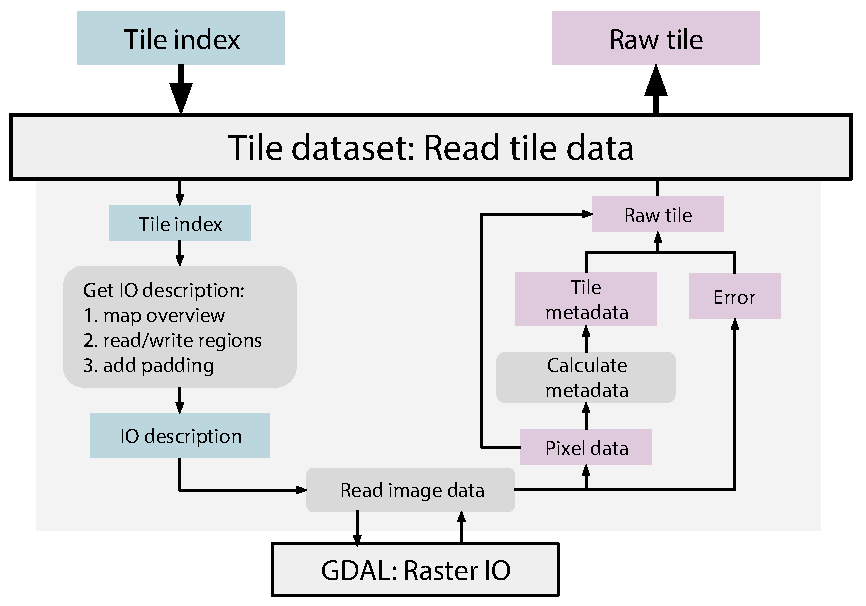
\includegraphics[width=\textwidth]{figures/implementation/pipeline/tiledataset.pdf}
    \end{subfigure}
    \caption{Tile datasets reads tiled pixel regions.}
    \label{fig:tiledataset}
\end{figure}

\subsubsection{Get IO Description}
The IO description contains all tile specific information needed to perform a map read request using GDAL. This includes the pixel region to read, and where to store the result. The derivation of this information is summarized in the following steps, and illustrated in Figure \ref{fig:getiodescription}.

\begin{figure}[htbp]
    \centering
    \begin{subfigure}[bt]{0.9\textwidth}
        \includegraphics[width=\textwidth]{figures/implementation/pipeline/getiodescription.pdf}
    \end{subfigure}
    \caption{Overview of the calculation of an IO description}
    \label{fig:getiodescription}
\end{figure}

\begin{enumerate}
\item Calculate a \class{Geodetic Patch} from \class{Tile Index}
\item Calculate the pixel coordinates for the patch in raster coordinate space
\item Calculate a suitable map overview
\item Transform pixel region to map overview
\item Add padding to the down scaled pixel region
\item Finalize the gathered data to an IO description object.
\end{enumerate}

In the scheme in Figure \ref{fig:getiodescription}, step one is performed using equation \ref{eq:latlongindex},

\begin{equation}
\label{eq:latlongindex}
\begin{split}
\phi_{NE} = 2\pi y / 2^{level} \\
\theta_{NE} = 2\pi x / 2^{level} \\
side = 2\pi / 2^{level},
\end{split} 
\end{equation}

where $\phi_{NE}$ and $\theta_{NE}$ are the latitude and the longitude of the north east corner of the tile and $side$ is the side length of the tile.

Calculating the corresponding GDAL overview is done according to equation \ref{eq:overview},

\begin{equation}
\label{eq:overview}
Overview(level) = N - level - 1 - log_2(size_{tile} / size_{map}),
\end{equation}

where $level$ is given by the provided \class{Tile Index}, $N$ is the total number of overviews in the dataset, $size_{tile}$ is a configurable constant defining the preferred pixel size of a tile and $size_{map}$ is the size of the full map in pixels. The sizes can be either along the $x-$ or $y-$ axis. In the implementation the $x-$axis is used.

Pixel coordinates can easily be transformed across map overviews using equation \ref{eq:overview}.

\begin{equation}
\label{eq:overview}
p_{n} = p_{m} \times 2^{m-n}
\end{equation}

Where $n$ is the destination map overview and $m$ is the source map overview. This is used for downscaling the pixel region in step 4, where $n$ is the calculated suitable overview and $m$ is zero (i.e. the full map). 

Padding is added to the pixel region in order to perform correct interpolation of pixel values across different tiles later during rendering. However, this may cause the pixel region to extend outside the map region. Therefore the last finalize step also handles wrapping of the pixel region before returning the final IO description. The wrapping used is a CPU implementation of $GL\_REPEAT$.

\subsubsection{Tile Meta Data}
As mentioned, \class{Tile Dataset}s can be configured to calculate some metadata on the fly based on the pixel data that has been read. The metadata includes minimum and maximum pixel values within the pixel data and whether or not the pixel data contains missing-data values. Having access to minimum and maximum values for height layer tiles is required for the culling to be performed correctly since the cullers rely on having bounding boxes for the chunks. The meta data can not be requested directly from GDAL since the tiling can differ from the underlying image tiling abstracted away by GDAL. Calculating the meta data had to be performed by explicitly looping through all the pixel values on the client side. 

\subsubsection{Summary}
To summarize, the implementation of \class{Tile Dataset} allow reading pixel data from a GDAL dataset corresponding to a specific \class{Tile Index}, along with metadata unless opted out. The \class{Raw Tile}s that are served are padded in order to perform smooth pixel blending between different tiles. \class{Raw Tile}s are not available for rendering since the data is not yet on the GPU.

\subsection{Async Tile Dataset}
\class{Async Tile Dataset}s utilize a shared thread pool and own a \class{Tile Dataset}. It provides a concurrent job posting interface for concurrent reads within the \class{Tile Dataset}. It has two important funcionalities: 1) enqueueing tile read jobs and 2) collect finished tile read jobs. Reading \class{Raw Tile}s on separate threads ensures that the render thread will not be delayed by image data requests, see Figure \ref{fig:asynctiledataset}.

\begin{figure}[htbp]
    \centering
    \begin{subfigure}[bt]{0.6\textwidth}
        \includegraphics[width=\textwidth]{figures/implementation/pipeline/asynctiledataset.pdf}
    \end{subfigure}
    \caption{Asynchronious reading of Raw tiles.}
    \label{fig:asynctiledataset}
\end{figure}

\begin{figure}[htbp]
    \centering
    \begin{subfigure}[bt]{0.6\textwidth}
        \includegraphics[width=\textwidth]{figures/implementation/pipeline/asynctiledataset_gettiles.pdf}
    \end{subfigure}
    \caption{Retrieving finished Raw tiles.}
    \label{fig:asynctiledataset2}
\end{figure}

The \class{Async Tile Dataset} internally keeps track of what tile indices it has enqueued and what tile pixel regions are currently being read. If a pixel region for a specific tile index is already enqueued or currently being read, the request is simply ignored. 


\section{Providing Tiles}
\class{Tile}s have three properties: a texture, metadata and a status. The status is used to report any type of problem with the tile. This includes IO errors, Out-of-range errors or simply Unavailable. Tiles that have the ``OK'' status however, are uploaded to the GPU and can be used for rendering. 

Tiles are provided for rendering through \class{Tile Provider}s. They define an interface that allow accessing tiles and meta data about the tiles. There are different types of tile providers, but they must all implement the following functionality:

\begin{itemize}
\item GetTile(\class{TileIndex}) - access the tile at the provided tile index.
\item GetDefaultTile() - returns a default tile with status ``OK''.
\item GetDepthTransform() - pixel value scale factor, e.g. for converting height map values to meters.
\item GetMaxLevel() - the highest mip level defined for the dataset.
\item GetNoDataValue() - get value that should be interpreted as ``no data''.
\item CheckTileStatus(\class{TileIndex}) - check tile status with no side effects.
\item Update() - called once per frame, allow for internal updates.
\item Reset() - full reset of internal state.
\end{itemize}

\begin{figure}[htbp]
    \centering
    \begin{subfigure}[bt]{0.4\textwidth}
        \includegraphics[width=\textwidth]{figures/implementation/tileprovider/tileprovider_gettile.pdf}
    \end{subfigure}
    \caption{Tile provider interface for accessing tiles.}
    \label{fig:tileprovider}
\end{figure}

The most important functionality is the GetTile ability, which is used by client code to access the tiles. As tile providers may provide tiles of any status, the user of the tile provider is responsible to always check the status of the requested tile before using the tile. 

Several implementations of the tile provider interface were developed. They are all described below.

\subsection{Caching Tile Provider}
\class{Caching Tile Provider} uses an \class{Async Tile Dataset} to read \class{Raw Tile}s as soon as client code tries to access a specific tile. It internally polls the \class{Async Tile Dataset} every frame for finished raw tiles. When there are ready raw tiles, the \class{Caching Tile Provider} converts the raw tiles into tiles. This is done in the initialization step which is part of the update method that is illustrated in figure \ref{fig:cachingtileprovider_update}. If no errors of the raw tile are reported, the tile gets the status ``OK'' and its texture data gets uploaded to the GPU. The tile also gets added to the in-memory cache. The functionality of accessing tiles is illustrated in Figure \ref{fig:cachingtileprovider_gettile}.

The uploading of texture data to the GPU needs to be done on the rendering thread since there is where the OpenGL context resides. Tiles with data uploaded to texture memory will enable it for use in rendering of a chunk.

\begin{figure}[htbp]
    \centering
    \begin{subfigure}[bt]{0.7\textwidth}
        \includegraphics[width=\textwidth]{figures/implementation/tileprovider/cachingtileprovider_gettile.pdf}
    \end{subfigure}
    \caption{Tiles are either provided from cache or requested.}
    \label{fig:cachingtileprovider_gettile}
\end{figure}

The functionality for internally updating the tile cache is illustrated in Figure \ref{fig:cachingtileprovider_update}.

\begin{figure}[htbp]
    \centering
    \begin{subfigure}[bt]{0.6\textwidth}
        \includegraphics[width=\textwidth]{figures/implementation/tileprovider/cachingtileprovider_update.pdf}
    \end{subfigure}
    \caption{The tile cache is updated once per frame.}
    \label{fig:cachingtileprovider_update}
\end{figure}

Figure \ref{fig:cachingtileprovider_tilerequest} demonstrates a typical scenario where a specific tile of index $\{3, 4, 2\}$ is requested within a sequence of render calls. The first requesting call to that tile will spawn a worker thread in the \class{Asynch Tile Dataset}. As soon as the \class{Tile} is initialized (uploaded to the GPU) and inserted in the cache, it will be accessible on the rendering thread. If the tile is not yet available the \class{Caching Tile Provider} will report that so that the calling function can continue without the use of that specific \class{Tile}.

\begin{figure}[htbp]
    \centering
    \begin{subfigure}[bt]{0.8\textwidth}
        \includegraphics[width=\textwidth]{figures/implementation/tileprovider/cachingtileprovider_tilerequest.pdf}
    \end{subfigure}
    \caption{Tiles are fetched on demand}
    \label{fig:cachingtileprovider_tilerequest}
\end{figure}

The caching policy implemented and used is LRU - ``Least Recently Used''. This means that tiles that have not been accessed for a while are thrown out only when the cache limit is exceeded, see section \ref{section:lrucaching} for details.

\subsection{Temporal Tile Provider}
In order to incorporate time-resolved map datasets into the rendering scheme, a tile provider for this specific purpose was implemented. The \class{Temporal Tile Provider} is instantiated with a template URI containing a time placeholder. Information about the supported time range, time resolution and expected timestamp format to be used in the template URI is also passed during instantiation. In Listing \ref{lst:temporal}, all tags starting with \texttt{OpenSpace} are used to configure information used to instantiate the temporal dataset. The tag \texttt{GDAL\_WMS} contains a functional GDAL WMS dataset specification. When requesting the URLs for the dataset, \texttt{\$\{OpenSpaceTimeId\}} will be replaced with the date and time in the specified format.

\begin{lstlisting}[language=XML,caption={Temporal WMS dataset specification.} \label{lst:temporal}]
<OpenSpaceTemporalGDALDataset>
    <OpenSpaceTimeStart>2015-11-24</OpenSpaceTimeStart>
    <OpenSpaceTimeEnd></OpenSpaceTimeEnd>
    <OpenSpaceTimeResolution>1d</OpenSpaceTimeResolution>
    <OpenSpaceTimeIdFormat>YYYY-MM-DD</OpenSpaceTimeIdFormat>
    <GDAL_WMS>
        <Service name="TMS">
            <ServerUrl>
                http://datasetURL/${OpenSpaceTimeId}/${z}/${y}/${x}.jpg 
            </ServerUrl>
        </Service>
        ...
    </GDAL_WMS>
</OpenSpaceTemporalGDALDataset>
\end{lstlisting}

At runtime, the \class{Temporal Tile Provider} checks the global simulation time, quantizes that time with respect to the provided time resolution and lazily instantiates new \class{Caching Tile Provider}s per timeframe within the temporal dataset. 

A schematic illustration of the implementation of the \class{Temporal Tile Provider} is illustrated in Figure \ref{fig:temporaltileprovider_gettile}.

\begin{figure}[htbp]
    \centering
    \begin{subfigure}[bt]{0.7\textwidth}
        \includegraphics[width=\textwidth]{figures/implementation/tileprovider/temporaltileprovider_gettile.pdf}
    \end{subfigure}
    \caption{Each temporal snapshot is internally represented by a caching tile provider.}
    \label{fig:temporaltileprovider_gettile}
\end{figure}


\subsection{Single Image Tile Provider}
This is a very simple implementation of the tile provider interface which only serves the same tile for every tile index. This tile provider was used for testing and debugging alignment and padding between tiles, see Figure \ref{fig:singleimagetileprovider_gettile}.

\begin{figure}[htbp]
    \centering
    \begin{subfigure}[bt]{0.5\textwidth}
        \includegraphics[width=\textwidth]{figures/implementation/tileprovider/singleimagetileprovider_gettile.pdf}
    \end{subfigure}
    \caption{Serving single tiles can be useful for debugging chunk and texture alignment.}
    \label{fig:singleimagetileprovider_gettile}
\end{figure}

\subsection{Text Tile Provider}
The ability to serve tiles with text rendered on the fly was implemented as a general debugging utility. The tiles are generated on demand by rendering text to textures and cached using the same LRU caching mechanism as the \class{Caching Tile Provider}.

\begin{figure}[htbp]
    \centering
    \begin{subfigure}[bt]{0.6\textwidth}
        \includegraphics[width=\textwidth]{figures/implementation/tileprovider/texttileprovider_gettile.pdf}
    \end{subfigure}
    \caption{Serving single tiles can be useful for debugging chunk and texture alignment.}
    \label{fig:texttileprovider_gettile}
\end{figure}

Two different types of \class{Text Tile Provider}s were implemented. \class{Tile Index Tile Provider} serves tiles where each tile has its tile index rendered onto it, and \class{Size Reference Tile Provider} uses the globe's reference ellipsoid to render a size reference in meters or kilometers onto its tiles.


\section{Mapping Tiles onto Chunks}
  
In the implementation of chunks suggested by Cozzi and Ring \cite{cozzi11}, chunks store the data they need for rendering by them selves. That means that as soon as a chunk has been fully initialized, it has everything it needs to be rendered. However, when dealing with multiple map datasets potentially residing on distant servers, there is no guarantee that all the tiles needed for a chunk to be rendered are available.

When an accessed \class{Tile} does not have the status ``OK'', it can not be used for rendering. The second best thing to try is to check the parent of the tile. A parent tile is guaranteed to always covers a larger geodetic map region that includes its children's subregions, but with lower number of pixels per geodetic degree. Figure \ref{fig:tiles} demonstrates this with a simple example.

\begin{figure}[htbp]
    \centering
    \begin{subfigure}[t]{0.3\textwidth}
        \includegraphics[width=\textwidth]{figures/implementation/chunktile/chunktile1.jpg}
        \caption{Requested tile.}
    \end{subfigure}
    \quad
    \begin{subfigure}[t]{0.3\textwidth}
        \includegraphics[width=\textwidth]{figures/implementation/chunktile/chunktile2.jpg}
        \caption{Requested tile's region shown in its parent tile.}
    \end{subfigure}
    \caption{Only the highlighted subset of the parent tile is used for rendering the chunk.}
    \label{fig:tiles}
\end{figure}

In figure \ref{fig:tiles}, it is realized that in order to use a parent tile for rendering, the texture coordinates used to sample the parent tile needs to be adjusted to represent the same geographic region. This shows the need of a higher level concept than just \class{Tile}s, which leads to the introduction of \class{Chunk Tile}s.

\subsection{Chunk Tiles}
  
A \class{Chunk Tile} represents a \class{Tile} that corresponds to a specific \class{Chunk}. It stores a \class{Tile} which is guaranteed to have the status ``OK'' along with a transform defined by a scaling and translation component. The transform is used to map texture coordinates of the chunk into its corresponding geodetic region within the tile. 

The algorithm used for selecting the highest resolution \class{Chunk Tile} from a tile provider is described by the pseudo code in Listing \ref{lst:getchunktile}.

\begin{lstlisting}[
  caption={Selecting optimal Chunk Tiles} 
  \label{lst:getchunktile}
]
ChunkTile TileSelector::getChunkTile(TileProvider* tp, TileIndex ti){
  TileUvTransform uvTransform;
  uvTransform.uvOffset = glm::vec2(0, 0);
  uvTransform.uvScale = glm::vec2(1, 1);

  while (ti.level > 1) {
      Tile tile = tp->getTile(ti);
      if (tile.status == Tile::Status::OK) {
          return { tile, uvTransform };
      }
      else {
        ascendToParent(ti, uvTransform);
      }
  }

  uvTransform.uvOffset = glm::vec2(0, 0);
  uvTransform.uvScale = glm::vec2(1, 1);
  return { Tile::TileUnavailable, uvTransform };
}
\end{lstlisting}

\iffalse
\begin{algorithm}[htp]
 \caption{Selecting optimal chunk tiles}
 \KwResult{ Chunk tile: \{Tile, UvTransform\}  }
  \SetKwProg{myalg}{GetChunkTile}{(tileProvider, tileIndex)}{}
  \myalg{}{
  \While {tileIndex.level > 0}{
      tile = tileProvider.getTile(tileIndex)
  }
  \eIf{(tile.status == OK)}{
        Return \{ tile, tileUvTransform \}
    }{
      tileUvTransform = fromParent(tileUvTransform, tileIndex);
      tileIndex.toParent();
    }
  }
  Return \{ tileProvider.defaultTile(), \{Translation: \{0,0\}, Scaling: \{1,1\} \} \}
  {}
  \label{alg:tileselection}
\end{algorithm}


\begin{algorithm}[htp]
\caption{Selecting optimal chunk tiles}
\label{alg:tileselection}
\KwResult{ A \class{ChunkTile} defined by a \class{Tile} and a \class{UvTransform}  }
  \SetKwProg{myalg}{GetChunkTile}{(\class{TileProvider}, \class{TileIndex})}{}
  \myalg{}{
    Initialize \class{UvTransform} with no scaling and no translation\\
    \While {level of \class{TileIndex} > 0}{
      Use \class{TileProvider} to access \class{Tile} at \class{TileIndex}\\
      \eIf{(\class{Tile} has status OK)}{
        \Return \class{ChunkTile} defined by \class{Tile} and \class{UvTransform}\\
      }{
        Modify \class{UvTransform} and \class{TileIndex} to represent the same geographic region at a higher mip level
      }
    }
    Use \class{TileProvider} to access the \class{Default Tile}\\
    Let \class{UvTransform} have no scaling and no translation\\
    \Return \class{ChunkTile} defined by \class{Default Tile} and \class{UvTransform}\\
  }
  {}
\end{algorithm}
\fi

 
The subroutine \texttt{ascendToParent} returns an updated transform which maps texture coordinates to the same geodetic region within the next parent tile. The routine is described in Listing \ref{lst:ascendtoparent}.

\begin{lstlisting}[caption={Ascend to parent} \label{lst:ascendtoparent}]
void TileSelector::ascendToParent(TileIndex& tileIndex, TileUvTransform& uv) {
    uv.uvOffset *= 0.5;
    uv.uvScale *= 0.5;

    if (tileIndex.isEastChild()) {
        uv.uvOffset.x += 0.5;
    }

    // In OpenGL, positive y direction is up
    if (tileIndex.isNorthChild()) {
        uv.uvOffset.y += 0.5;
    }

    tileIndex.toParent();
}
\end{lstlisting}

\iffalse
\begin{algorithm}[htp]
 \caption{Get the transform from the parents texture coordinates}
 \KwResult{ UvTransform: \{Translation, Scaling\}  }
  \SetKwProg{myalg}{fromParent}{(tileUvTransform, tileIndex)}{}
  \myalg{}{
      tileUvTransform.translation *= 0.5
      tileUvTransform.scaling *= 0.5
  \If{(tileIndex is an eastern child)}{
        tileUvTransform.translation.x += 0.5
    }
    \If{(TileIndex is a northern child)}{
        tileUvTransform.translation.y += 0.5
    }
  }
  Return tileUvTransform
  {}
  \label{alg:fromparent}
\end{algorithm}

The subroutine \texttt{getParent} simply returns the parent of the provided tile index as described in Algorithm \ref{alg:parent}.

\begin{algorithm}[htp]
 \caption{Get the parent tile index}
 \KwResult{ TileIndex: \{level, x, y\}  }
  \SetKwProg{myalg}{TileIndex::Parent}{}{}
  \myalg{}{
  Return \{level-1, x/2, y/2\}
  }{}
  \label{alg:parent}
\end{algorithm}
\fi

As opposed to regular tiles, chunk tiles can always be used for rendering since they by definition always have the status ``OK''.

\subsection{Chunk Tile Pile}
\label{section:chunktilepile}

A \class{Chunk Tile Pile} represents a range of \class{Chunk Tile}s across multiple mip levels. They contain the information needed to perform the LOD switching later described under section \ref{section:lodswitching}. Retrieving a \class{Chunk Tile Pile} simply requires a tile index of the highest desired mip level (highest LOD) and the number of desired \class{Chunk Tile}s in the pile as described in Listing \ref{lst:chunktilepile}.

\iffalse
\begin{algorithm}[htp]
 \caption{Get a chunk tile for a specific tile index}
 \KwResult{ ChunkTilePile }
  \SetKwProg{myalg}{getChunkTilePile}{(tileProvider, tileIndex, pileSize)}{}
  \myalg{}{
  chunkTilePile = [ ] \\
  \For{i in range [1, pileSize]}{
  	chunkTilePile.append(getChunkTile(tileIndex)) \\
  	tileIndex = tileIndex.parent()
  }
  Return chunkTilePile
  }{}
  \label{alg:getchunktilepile}
\end{algorithm}
\fi

\begin{lstlisting}[caption={Instantiating a Chunk Tile Pile} \label{lst:chunktilepile}]
ChunkTilePile TileSelector::getChunkTilePile(TileProvider* tp, TileIndex ti, int n){
  ChunkTilePile chunkTilePile;
  for (int i = 0; i < n; ++i){
    chunkTilePile.push_back(getChunkTile(tp, ti));
    ti.toParent();
  }
  return chunkTilePile;
}
\end{lstlisting}

As an example: 
Assuming that the texture data is available in local memory, invoking the getChunkTilePile method with index $\{x: 2240, y: 4824, level: 13 \}$ and a chunk tile pile size 3, would return the \class{Chunk Tile Pile} represented in Figure \ref{fig:chunktilepile}. 

\begin{figure}[htbp]
    \centering
    \begin{subfigure}[t]{0.3\textwidth}
        \includegraphics[width=\textwidth]{figures/implementation/chunktile/chunktilepile3.png}
        \caption{Tile.}
    \end{subfigure}
    \quad
    \begin{subfigure}[t]{0.3\textwidth}
        \includegraphics[width=\textwidth]{figures/implementation/chunktile/chunktilepile2.png}
        \caption{Parent 1.}
    \end{subfigure}
    \quad
    \begin{subfigure}[t]{0.3\textwidth}
        \includegraphics[width=\textwidth]{figures/implementation/chunktile/chunktilepile1.png}
        \caption{Parent 2.}
    \end{subfigure}
    \caption{Only the highlighted subset of the parent tiles are used for rendering the chunk.}
    \label{fig:chunktilepile}
\end{figure}

As chunk tiles are guaranteed to be good for rendering on the GPU (since their tiles are guaranteed to have the status ``OK''), all \class{Chunk Tile Pile}s are guaranteed to be good for rendering as well. 

\section{Managing Multiple Data Sources}
The \class{Layer Manager} maintains and organizes different types of texture data sources into groups. This is required as different types of texture datasets are used for different purposes and thus rendered in different ways. The \class{Layer Manager} owns seven \class{Layer Groups}; these are:

\begin{enumerate}
\item Heightmaps
\item ColorLayers
\item ColorOverlays
\item GrayScaleLayers
\item GrayScaleOverlays
\item NightLayers
\item WaterMasks
\end{enumerate}

\subsection{Layers}
Much like in image editing softwares, a layer in this context represents a raster of pixels, which among other internally ordered raster of pixels, are used to produce a final result. A \class{Layer} consists of three things:

\begin{enumerate}
\item A \class{Tile Provider} - Used for accessing tiles of texture data.
\item A collection of render settings for real time image processing. The parameters implemented at this stage are \emph{gamma}, \emph{multiplier} and \emph{opacity}.
\item A simple boolean property which specifies whether the layer is enabled or disabled. Disabled layers are not used in rendering.
\end{enumerate}

\class{Layer}s allow for retrieving of \class{Chunk Tile Pile}s, as described in section \ref{section:chunktilepile}. The class hierarchy and data flow is illustrated in Figure \ref{fig:layermanager}.

\begin{figure}[htbp]
    \centering
    \includegraphics[width=\textwidth]{figures/implementation/layers/layermanager.pdf}
    \caption{UML diagram of the \class{Layer Manager} and its related classes.}
    \label{fig:layermanager}
\end{figure}

\subsection{Layers on the GPU}

The data hierarchy defined by \class{Layer Manager} can almost be reproduced on the GPU by using GLSL in a near object-oriented approach. In order to handle the data mapping between the CPU and GPU, a CPU representation for the GPU data was implemented. This allows for updating the values of uniform variables and map uniform names to uniform locations.

\subsubsection{CPU to GPU Data Mapping}

There are some key differences between the \class{Layer Manager} data structure on the CPU and its corresponding GPU-synchronized representation - \class{GPU Layer Manager}. These are:

\begin{itemize}
\item The GPU representation does not store any of the actual \class{Layer} data - only the uniform locations within a shader program so that it knows where to upload the layer data to the GPU. 
\item Render calls are done on a per chunk basis. This means that all texture data to be used within a single render call is contained in a single \class{Chunk Tile Pile} for each \class{Layer}. Thus, the \emph{provides}-relation between \class{Layer} and \class{Chunk Tile Pile} in Figure \ref{fig:layermanager} simply becomes a \emph{has}-relation between a \class{GPU Layer} and a \class{GPU Chunk Tile Pile}.
\item Layers that are disabled are not rendered, and consequently not uploaded to the GPU. This means that all layers on the GPU are enabled, thus they do not need to store that information.
\end{itemize}

Incorporating these few differences yields a similar class hierarchy, as illustrated in Figure \ref{fig:gpulayermanager}. 

\begin{figure}[htbp]
    \centering
    \includegraphics[width=\textwidth]{figures/implementation/layers/gpulayermanager.pdf}
    \caption{UML structure for corresponding GPU-mapped hierarchy. The class \texttt{GPUData<T>} maintains an OpenGL uniform location.}
    \label{fig:gpulayermanager}
\end{figure}

The leaf classes within the class hierarchy store one uniform location each and represent one GLSL uniform value. The declaration of the layer uniforms within the shader code is defined so that it matches the exact same hierarchy. This is implemented by mapping C++ classes to GLSL structs and representing \emph{one-to-many} relationships as structs with a range of conformly named fields, or plain GLSL arrays.

\subsubsection{Updating the GPU Data}

With this 1:1 data mapping between the CPU and GPU, all the GPU-prefixed classes were given two responsibilities.

\begin{enumerate}
\item Bind its uniform locations to GLSL variable names within a provided shader program.
\item Set its uniform values within a provided shader program. That is, a \class{GPU Chunk Tile} should be able to set its uniform values from a regular \class{ChunkTile}.
\end{enumerate}

The leaf classes automatically takes care of both binding its uniform location to specific GLSL variables and  setting their uniform values. The compound GPU-prefixed classes (non leaf classes) more or less simply propagates the method calls to all its dependents. When binding an object to a variable name, the GLSL variable identifiers are built up successively during the propagation down to the leaf classes. \class{GPU Layer} is used as an example in Listing \ref{lst:bindgpulayer}.

\begin{lstlisting}[
  caption={Bind a GPU Layer to a Layer on the CPU} 
  \label{lst:bindgpulayer}
]
void GPULayer::bind(ProgramObject* p, std::string nameBase, int pileSize){
	this->gpuChunkTilePile.bind(p, nameBase + "pile.", pileSize)
	this->gpuRenderSettings.bind(p, nameBase + "settings.")
}
\end{lstlisting}

In Listing \ref{lst:bindgpulayer}, it can be concluded that each layer in the GLSL code must be a struct with a member called ``pile'' and a member called ``settings''. An example of a fully resolved identifier is: 

\begin{lstlisting}[]
"ColorLayers[0].pile.chunkTile0.tileUvTransform.scaling"
\end{lstlisting}

When setting the values, the GPU representation of the data is updated based on the currently available \class{Layer} data, and the update is propagated down to all the leaf classes. This is exemplified using code from the \class{GPULayer} class defined in Listing \ref{lst:gpulayersetvalue}.

\begin{lstlisting}[
  caption={Set all GPU Layer variables from a CPU Layer} 
  \label{lst:gpulayersetvalue}
]
GPULayer::setValue(ProgramObject* p, Layer& l, TileIndex ti, int n){
	ChunkTilePile chunkTilePile = l.getChunkTilePile(ti, n);
	this->gpuChunkTilePile.setValue(p, chunkTilePile);
	this->gpuRenderSettings.setValue(p, l.renderSettings());
}
\end{lstlisting}

\section{Chunk Rendering}

Given the ability to specify and use different layers to be used for rendering and the actual chunks that need to be visible, they are ready to be rendered. Rendering includes using vertex- and fragment shaders when invoking a rendering call on a given geometry; in this case, a grid.

\subsection{Grid}

A chunk grid is defined by a number of segments N in two dimensions, which is used to build up a two dimensional array of vertex coordinates. These vertex coordinates can be used both for texture fetching and as interpolation parameters in an inverse geographic projection function to place a each vertex in 3D space. Figure grid shows how a surrounding region have coordinate values less than 0 or greater than 1 in either the u or the v dimension. This region is referred to as the skirt of the grid and it is offset in the vertical direction in the vertex shaders to cover cracks between chunks.

\begin{figure}[htbp]
    \centering
    \includegraphics[width=0.5\textwidth]{figures/implementation/rendering/grid.pdf}
    \caption{Grid with skirts.}
    \label{fig:grid}
\end{figure}

\subsection{Vertex Pipeline}

The grid can be rendered using different methods to weight precision against accuracy. In the vertex shader, the vertex positions are set so that the chunk geometry can be rasterized and rendered as a mesh on the screen. Height mapping is performed by offsetting vertices in the direction of the geodetic normals on the GPU which means that vertex texture fetching is needed in the rendering pipeline.

The mapping from geodetic coordinates to cartesian model space coordinates can be done on the GPU in single precision to position vertices on the globe. As discussed in section \ref{section:precision}, however, this is not sufficient to achieve sub meter precision on an Earth sized globe.

\subsubsection{High Precision Rendering}

The first step in avoiding precision errors is what Cozzi and Ring refers to rendering relative to center \cite{cozzi11}. In short, it boils down to calculating the model-view matrix in double precision on the CPU side and then casting the matrix to a single precision representation before uploading it to the GPU. This method works well for small objects where the vertices positioned close to the origin (center) of the model \cite{cozzi11}. For planet sized objects, we need to go further than that.

One method that works for all models but can be considered naive as the number of vertices increases is what Cozzi and Ring refers to as CPU relative to eye rendering. By using a dynamic vertex buffer, all vertex positions can be transformed to camera space in double precision before being cast to single precision and dynamically uploaded to the GPU. This method becomes very tedious if the number of vertices is big. However, since the mesh of a chunk is essentially an ellipsoid segment, the whole mesh can be interpolated using a limited number of control points.

We have considered two different categories of rendering techniques: model space rendering and camera space rendering. The techniques can be implemented differently and used at different scales to accommodate for flexibility, accuracy and precision.

\subsubsection{Model Space Rendering}

The most straightforward method for rendering geodetic chunks is to transform the geodetic coordinates of each vertex to cartesian model space coordinates using the inverse geographic projection transform, $P^{-1}(\phi, \theta)$, in the vertex shader. An affine transform can be applied to the vertex coordinates by knowing the geodetic coverage of the chunk. It can be derived from the chunk's tile index. The inverse projection transform is performed with limited precision floating point operations on the GPU but the accuracy will be high as vertices will be positioned exactly on the globe in geodetic coordinates. Figure \ref{fig:global}.

\begin{figure}[htbp]
    \centering
    \begin{subfigure}[tb]{0.3\textwidth}
    	\includegraphics[width=\textwidth]{figures/implementation/rendering/gridmap.pdf}
    \end{subfigure}
    \begin{subfigure}[tb]{0.4\textwidth}
    \begin{picture}(50,50)
        \put(25,25){$\left( \begin{matrix} x \\ y \\ z \end{matrix} \right) =P^{ -1 }(\phi ,\theta )\rightarrow$}    
    \end{picture}
    \end{subfigure}
    \begin{subfigure}[tb]{0.2\textwidth}
    	\includegraphics[width=\textwidth]{figures/implementation/rendering/gridonglobe.png}
    \end{subfigure}
    \caption{Model space rendering of chunks is performed with a mapping of vertices from geodetic coordinates to cartesian coordinates.}
    \label{fig:global}
\end{figure}

The model space rendering method essentially achieves the same precision as rendering a predefined chunk mesh relative to the center of mass of the globe. Figure \ref{fig:pipelineglobal} shows the pipeline for rendering a chunk using the model space method. Variables on the CPU are defined in double precision and cast to single precision before being uploaded to the GPU.

\begin{figure}[htbp]
    \centering
    \includegraphics[width=\textwidth]{figures/implementation/rendering/pipeline_global.pdf}
    \caption{Vertex pipeline for model space rendering.}
    \label{fig:pipelineglobal}
\end{figure}

\subsubsection{Camera Space Rendering}

Camera space rendering is performed by transforming only a limited number of control points for each chunk to camera space using double precision arithmetics. Once in camera space, the points can be cast to single precision and used for interpolation on the GPU to get all the final vertex positions of the chunk. Having the points in camera space solves the proposed precision issues since the precision will increase when the points are closer to the camera. This concept is illustrated in Figure \ref{fig:local} where the vertex position vector precision increases as vertices are closer to the camera.

\begin{figure}[htbp]
    \centering
    \includegraphics[width=0.5\textwidth]{figures/implementation/rendering/local.pdf}
    \caption{Interpolating vertex positions in camera space leads to high precision in the representation of vertex positions close to the camera compared to positions defined in model space.}
    \label{fig:local}
\end{figure}

\paragraph{Chunks as NURBS Surfaces}
Non Uniform Rational B-Splines (NURBS) can represent all conic sections exactly which is important for modelling ellipses in the 1D case and ellipsoids in the 2D case. A geodetic chunk can be uniquely defined by nine control points which can be calculated using the tile index representing the chunk.

The positive aspect about rendering geodetic chunks as NURBS surfaces is that it is a unified way of rendering chunks and that the precision works for all scales. Chunks will always be mapped exactly on the ellipsoid and the precision will increase when the camera gets closer. However, the negative aspect that makes NURBS insufficient for texture mapped globes is the fact that the texture coordinates of the vertices do not linearly map to the geodetic coordinates of the chunk. In other words, vertices are not evenly distributed along the surface of the chunk which leads to distorted textures. The reason for this is the fact that NURBS are rational parametric functions. For example, a circle segment can be represented exactly but a given parameter value will not yield the same position along a circle segment as a circle segment parameterized as $(x(t),y(t)) = (cos(t), sin(t))$. The $cos$ and $sin$ functions are irrational and can therefore not be represented with NURBS segments which by definition are rational.

\paragraph{Chunks as Bilinear Surfaces}
To avoid both the texture distortion of NURBS and the precision issues of model space rendering, we use a different method for rendering chunks that are closer to the camera and hence require higher precision. When the camera gets closer to the surface of the ellipsoid, the chunks will split and get smaller according to the chunk selection under Section \ref{section:chunkselection}. Smaller patches will automatically be better approximated as flat surfaces so that at a certain level, before the precision errors of the global patches become predominant, the rendering of patches can be switched to the a camera space rendering method which uses bilinear interpolation of vertex positions.

This method is performed by, just as in the case of NURBS surfaces, transforming control points from cartesian model space to camera space where they can be cast to single precision representations. Instead of NURBS interpolation, a simple bilinear interpolation is used to place all the vertices on the surface defined by the four corner points of the patch that covers the chunk.

With bilinear interpolation, high precision is achieved for vertices placed close to the camera. Also, the vertices will be uniformly spaced which means that the textures will not be distorted. Worth noticing is that if bilinear interpolation rendering is performed on chunks with low level, the approximation will be less accurate. Switching to camera space rendering with bilinear interpolation at level 10 gives a reasonable balance between the ellipsoidal mapping of the model space rendering and the high precision of the camera space chunk rendering.

Figure \ref{fig:pipelinelocal} shows a flowchart of the local vertex rendering pipeline. Variables on the CPU are defined in double precision and cast to single precision before being uploaded to the GPU.

\begin{figure}[htbp]
    \centering
    \includegraphics[width=\textwidth]{figures/implementation/rendering/pipeline_local.pdf}
    \caption{Vertex pipeline for camera space rendering.}
    \label{fig:pipelinelocal}
\end{figure}

\subsection{Fragment Pipeline}

The purpose of layered texture rendering is to provide the user an ability to toggle different kinds of layers for rendering a chunk. For each fragment, the final color is calculated by using the active layer groups. This is done using the following step in the fragment shader which is the same for the camera space rendered chunks as it is for the model space rendered chunks:


\begin{enumerate}
\item \textbf{For all ColorLayers}: Sample RGB, apply layer settings and update fragment RGBA using alpha blending.
\item \textbf{For all GrayscaleLayers}: Sample the grayscale value R, apply layer settings and update fragment V in color space HSV using alpha blending.
\item \textbf{For all GrayscaleOverlays}: Sample grayscale value R and A, apply layer settings and update fragment RGBA using alpha blending.
\item \textbf{For all WaterMasks}: Sample A, apply layer settings and add A as a specularity component for the fragment.
\item \textbf{For all NightTextures}: Sample RGB, apply layer settings and update fragment RGBA using alpha blending in shaded regions of the globe.
\item Perform shading by darkening shaded regions.
\item Add simple atmosphere color to RGB.
\item \textbf{For all ColorOverlays}: Sample RGBA, apply layer settings and update fragment RGBA using alpha blending.

\end{enumerate}

All of these steps are optional and can be toggled by activating or deactivating layers or specifying whether or not to perform shading or use atmosphere for rendering. Sampling the color from a layer group is done by looping through all layers in that group, see Listing \ref{lst:loopthroughlayers}. Listing \ref{lst:gettexval1} and \ref{lst:gettexval2} shows how layer weights and texture transforms for chunk tile piles are used for sampling of the tile textures. Layer settings is performed for all raster bands within all layers. The application of layer settings is shown in Listing \ref{lst:performsettings}.

\begin{lstlisting}[
  caption={Setting color for a given layer group. Example using ColorLayers.} 
  \label{lst:loopthroughlayers}
]
#for i in 0..#{lastLayerIndexColorLayers} {
		vec4 colorSample = getTexVal(ColorLayers[#{i}].pile,
			levelWeights, uv);
		colorSample = performLayerSettings(colorSample,
			ColorLayers[#{i}].settings);
		color = blendOver(color, colorSample); // Alpha blending
	}
#endfor
\end{lstlisting}

\begin{lstlisting}[
  caption={Getting texture value by blending a chunk tile pile.} 
  \label{lst:gettexval1}
]
vec4 getTexVal(ChunkTilePile chunkTilePile, LevelWeights w, vec2 uv){
	return w.w1 * getTexVal(chunkTilePile.chunkTile0, uv) + 
		w.w2 * getTexVal(chunkTilePile.chunkTile1, uv) + 
		w.w3 * getTexVal(chunkTilePile.chunkTile2, uv);
}
\end{lstlisting}

\begin{lstlisting}[
  caption={Using texture transform and sampling a texture.} 
  \label{lst:gettexval2}
]
vec4 getTexVal(ChunkTile chunkTile, vec2 tileUV){
	vec2 samplePosition = TileUVToTextureSamplePosition(chunkTile, tileUV);
	vec4 texVal = texture(chunkTile.textureSampler, samplePosition);
	return texVal;
}
\end{lstlisting}


\begin{lstlisting}[
  caption={Perform layer settings.} 
  \label{lst:performsettings}
]
float performLayerSettings(float currentValue, const LayerSettings settings) {
	float newValue = currentValue;
	newValue = sign(newValue) * pow(newValue, settings.gamma);
	newValue = newValue * settings.multiplier;
	newValue = newValue * settings.opacity;
	return newValue;
}
\end{lstlisting}

\subsection{Dynamic Shader Programs}

The ability to dynamically toggle layers with dynamic blending requires multiple sampling of textures in the fragment shaders. To avoid unnecessary processing when not all layers are in use there is a need to dynamically recompile the shader programs as layers are toggled. We use the GLSL preprocessor in the General Helpful Open Utility Library (GHOUL) \cite{ghoul} to preprocess all shader programs when the number of layers in use change.

We define a layer shader program to be a GLSL program object using vertex and fragment shading. Moreover, it fits the pipeline of rendering a chunk with a specific number of layer groups and a varying number of layers for each group.

To decide whether or not a layer shader program needs to be preprocessed and re-compiled, the relevant Layer Shader Preprocessing Data is saved for the layer shader program and compared to the updated preprocessing data if it has been changed by the user. Table \ref{table:layergrouppreprocessingdata} shows what data is needed to preprocess layer shader programs. Key-value pairs can be used to set properties that are used on a per-globe basis. Examples are \textbf{performShading} : \emph{true} or \emph{false}, \textbf{useAtmosphere} : \emph{true} or \emph{false}. Letting the preprocessor handle these properties avoids the need of uniform variable uploading and GLSL if-statements. The preprocessor also handles unrolling of for-loops which go through all layers in a group, see Listing \ref{lst:loopthroughlayers}.


\begin{table}
\centering 
\caption[]{Data used for a layer group for preprocessing of layer shader programs.}
\label{table:layergrouppreprocessingdata}
\begin{tabular}{ c }    
    	\hline
        \textbf{Layer Group Preprocessing Data} \\ 
    	\hline
	Number of layers: integer \\
    	Blending enabled: boolean \\
	\hline
\end{tabular}
\end{table}

\begin{table}
\centering
\caption[]{Data used for a renderable globe for preprocessing of layer shader programs.}
\label{table:layergrouppreprocessingdata}
\begin{tabular}{ c }
    
    	\hline
        \textbf{Layer Shader Preprocessing Data} \\ 
    	\hline
	0..* Preprocessing data: Layer Group Preprocessing Data \\
    	0..* Key-value pairs: pair of strings \\
    	\hline
    
\end{tabular}
\end{table}

\subsection{LOD Switching}
\label{section:lodswitching}
Instead of the time based switching routine proposed by Cozzi and Ring \cite{cozzi11}, we perform a distance based switching which works on a per fragment basis for textures and on a per vertex basis for height maps. The method is implemented in the vertex and fragment shaders and uses linear interpolation between levels. The blending technique introduces the concept of Chunk Tile Piles as seen in section \ref{section:chunktilepile}. A Chunk Tile Pile contains three chunk tiles of different level to achieve level blending which is used to avoid popping artefacts. 

When rendering a specific fragment of a chunk, blending between up to three chunk levels can be used as a part of the switching in the chunked LOD algorithm. Assuming that the level of Tile 0 is equal to the level of the chunk to render and that Chunk Tile 1 and Chunk Tile 2 are 1 and 2 levels lower respectively, three level weights can be determined based on the distance to the fragment to achieve smooth transitions between levels. The three level weights are based on an interpolation parameter $t$ as in Listing \ref{lst:levelweights}.

\begin{lstlisting}[
  caption={Calculate level weights.} 
  \label{lst:levelweights}
]
LevelWeights getLevelWeights(float t){ // level interpolation parameter
	LevelWeights levelWeights;
	levelWeights.w1 = clamp(1 - t, 0 , 1);
	levelWeights.w2 = clamp(t, 0 , 1) - clamp(t - 1, 0 , 1);
	levelWeights.w3 = clamp(t - 1, 0 , 1);
	return levelWeights;
}
\end{lstlisting}

The interpolation parameter $t$ is calculated using the distance to the camera $d$ and the current level of the chunk $l$ as in equation \ref{eq:interpolation}.

\begin{equation}
\label{eq:interpolation}
t = l-log_2(\frac{s}{d})
\end{equation}

where $s$ is a scale factor determining how much of the higher level tile to use in the blending. In the ideal case, the interpolation parameter should be a value between 0 and 1. However, adjacent chunks can have a difference in level greater than 1 which in turn leads to interpolation parameters with larger values. This is why it is not enough with two Chunk Tiles per Chunk Tile Pile to guarantee no popping. Popping can also occur if the LOD scale factor $s$ is small enough for adjacent chunks to have even bigger difference in level. Figure \ref{fig:blending} shows how the interpolation parameter from the desired level is used for blending between tiles of different level.

\begin{figure}[htbp]
    \centering
    \begin{subfigure}[tb]{0.49\textwidth}
    	\includegraphics[width=\textwidth]{figures/implementation/rendering/blending1.pdf}
	\caption{Blending disabled.}
    \end{subfigure}
    \begin{subfigure}[tb]{0.49\textwidth}
    	\includegraphics[width=\textwidth]{figures/implementation/rendering/blending2.pdf}
	\caption{Blending enabled.}
    \end{subfigure}
    \caption{Blending on a per fragment basis.}
    \label{fig:blending}
\end{figure}

\section{Interaction}

An interaction mode specifically for globe browsing had to be implemented to deal with the vast scale differences and limitations of camera movements required for browsing globes. 

Representing the camera state as a three dimensional cartesian vector for the position and a quaternion for the rotation made it possible to achieve interaction solving the proposed objectives. Basic linear algebra was used on vectors such as the geodetic normal of the globe in the camera position geodetically projected on the surface, camera position and direction as well as the height offset of the terrain.

The horizontal movement interaction speed was set to be proportional to the distance from the camera to the terrain surface. That way the user can come in close and slowly hover across the detailed terrains as well as quickly moving from one continent to the other by increasing the height to the surface.

The camera rotation quaternion can be decomposed in to two rotations; one directing the camera in the direction of the geodetic normal, and one directing it in the remaining view direction with a given roll. This way it is possible to both travel across the surface and keeping the horizon angle as well as looking around at the spot.

The camera is always pushed up above the surface of the terrain to avoid penetrating it. The minimum height given in meters can be set together with other parameters such as sensitivity and friction.

\chapter{Results}
This section goes through how the final implementation results in a software that solves the proposed objectives. Section (ref screenshots) includes screenshots showing the globe browsing in use.

The benchmarks were done using an relatively old consumer laptop computer. Its specs are provided below.

\begin{table}[h]
  \centering
  \caption[]{Computer used for Benchmarking}
    \label{table:benchmark host}
  \begin{tabular}{| r l |}
    \hline
      \textbf{Computer Model:}  & MacBook Pro (15'' early 2011) \\
      \textbf{Processor:}       & 2GHz Intel Core i7 \\
      \textbf{RAM:}             & 8 GB 1333MHz DDR3 RAM \\
      \textbf{Graphics:}        & AMD Radeon HD 6490M 256 MB \\
    \hline
  \end{tabular}
\end{table}

\clearpage
\section{Zooming In}
\FloatBarrier
The chunk rendering algorithm was evaluated for a top down view at different distances to the ground. The settings for the evaluation are presented in Table \ref{table:settingstopdown}, the camera views for the evaluation points are shown in Figure \ref{fig:topdown} and the results are presented in Figure \ref{fig:topdowngraph}.
\begin{table}[h]
  \centering
  \caption[]{Top down settings}
    \label{table:settingstopdown}
  \begin{tabular}{| r l |}
    \hline
      \textbf{Globe:}             & Earth \\
      \textbf{Map datasets:}      & HeightLayers=[GCS\_Elevation\footnote{http://services.arcgisonline.com/ArcGIS/rest/services/ESRI\_Imagery\_World\_2D/MapServer}] \\
                                  & ColorLayers=[ESRI\_World\_2D\footnote{http://198.102.45.23/arcgis/rest/services/worldelevation3d/terrain3d?}] \\
      \textbf{LOD Scale factor:}  & 10.0 \\
      \textbf{LOD Evaluation:}    & By distance \\
      \textbf{Culling:}           & Frustum culling, Horizon culling \\
      \textbf{Level blending:}    & Enabled \\
      \textbf{Camera View:}       & Facing down, varying altitudes\\
    \hline
  \end{tabular}
\end{table}

\begin{figure}[h]
    \centering
    \begin{subfigure}[bt]{0.31\textwidth}
        \includegraphics[width=\textwidth]{figures/results/topdown/topdown5.png}
        \caption{Earth}
    \end{subfigure}
    ~
    \begin{subfigure}[bt]{0.31\textwidth}
        \includegraphics[width=\textwidth]{figures/results/topdown/topdown4.png}
        \caption{East America}
    \end{subfigure}
    ~
    \begin{subfigure}[bt]{0.31\textwidth}
        \includegraphics[width=\textwidth]{figures/results/topdown/topdown3.png}
        \caption{New York City}
    \end{subfigure}
    ~
    \begin{subfigure}[bt]{0.31\textwidth}
        \includegraphics[width=\textwidth]{figures/results/topdown/topdown2.png}
        \caption{Manhattan}
    \end{subfigure}
    ~
    \begin{subfigure}[bt]{0.31\textwidth}
        \includegraphics[width=\textwidth]{figures/results/topdown/topdown1.png}
        \caption{Central Park}
    \end{subfigure}
    \caption{Top-down views of Earth at different zoom levels}
    \label{fig:topdown}
\end{figure}

\begin{figure}[h]
\begin{tikzpicture}
    \begin{axis}[
        width  = 1.0*\textwidth,
        height = 12cm,
        major x tick style = transparent,
        ybar=2*\pgflinewidth,
        bar width=8pt,
        ymajorgrids = true,
        %ylabel = {Number of},
        symbolic x coords={Earth, East America, NYC, Manhattan, Central Park},
        xtick = data,
        scaled y ticks = false,
        enlarge x limits=0.25,
        ymin=0,
        legend cell align=left,
        legend style={
                at={(0.43, 0.66)},
                anchor=south east,
                column sep=1ex
        }
    ]

      \addplot[style={chunks_color,fill=chunks_color,mark=none}]
        coordinates { (Earth, 10) (East America, 70) (NYC, 70) (Manhattan, 110) (Central Park, 142) };

      \addplot[style={leafs_color,fill=leafs_color,mark=none}]
        coordinates { (Earth, 8) (East America, 53) (NYC, 53) (Manhattan, 83) (Central Park, 107) };
      
      \addplot[style={rendered_color,fill=rendered_color,mark=none}]
        coordinates { (Earth, 7) (East America, 14) (NYC, 13) (Manhattan, 17) (Central Park, 11) };

      \addplot[style={globe_render_time,fill=globe_render_time,mark=none}]
        coordinates { (Earth, 17) (East America, 20) (NYC, 20) (Manhattan, 21) (Central Park, 21) };

      \addplot[style={frame_render_time,fill=frame_render_time,mark=none}]
        coordinates { (Earth, 1.1) (East America, 3.4) (NYC, 3.5) (Manhattan, 5) (Central Park, 5.6) };

      \legend{Chunks, Leaf chunks, Rendered chunks, Frame time [ms], Globe render time [ms]}

    \end{axis}
\end{tikzpicture}
\caption{}
\label{fig:topdowngraph}
\end{figure}



\clearpage
\section{Culling for distance based LOD}
\FloatBarrier
The culling algorithms Frustum culling and Horizon Culling were compared and evaluated. The settings used are provided in Table \ref{table:cullingd}. Note that LOD evaluation is done by distance. Figure \ref{fig:cullingdcam} shows the camera view evaluated. Figure \ref{fig:cullingd} shows and overview of the rendered chunks using the different culling and benchmarks are listed in Table \ref{table:cullingd}.

\begin{table}[h]
  \centering
  \caption[]{Culling test}
    \label{table:cullingd}
  \begin{tabular}{| r l |}
    \hline
      \textbf{Globe:}             & Earth \\
      \textbf{Map datasets:}      & HeightLayers=[GCS\_Elevation\footnote{http://services.arcgisonline.com/ArcGIS/rest/services/ESRI\_Imagery\_World\_2D/MapServer}] \\
                                  & ColorLayers=[ESRI\_World\_2D\footnote{http://198.102.45.23/arcgis/rest/services/worldelevation3d/terrain3d?}] \\
      \textbf{LOD Scale factor:}  & 7.8 \\
      \textbf{LOD Evaluation:}    & By distance \\
      \textbf{Culling:}           & \textbf{Evaluated} \\
      \textbf{Level blending:}    & Enabled \\
      \textbf{Camera View:}       & Looking towards western horizon\\
      \textbf{Location:}          & New York, New Jersey\\
    \hline
  \end{tabular}
\end{table}

\begin{figure}[h]
    \centering
    \begin{subfigure}[bt]{1.0\textwidth}
        \includegraphics[width=\textwidth]{figures/results/culling/cam_d.png}
    \end{subfigure}
    \caption{Camera view looking over Brooklyn, Manhattan and New Jersey with distance based LOD}
    \label{fig:cullingdcam}
\end{figure}

\clearpage
\begin{figure}[h]
    \centering
    \begin{subfigure}[bt]{0.48\textwidth}
        \includegraphics[width=\textwidth]{figures/results/culling/d.png}
        \caption{No culling}
    \end{subfigure}
    ~
    \begin{subfigure}[bt]{0.48\textwidth}
        \includegraphics[width=\textwidth]{figures/results/culling/df.png}
        \caption{Frustum culling}
    \end{subfigure}
    ~
    \begin{subfigure}[bt]{0.48\textwidth}
        \includegraphics[width=\textwidth]{figures/results/culling/dh.png}
        \caption{Horizon culling}
    \end{subfigure}
    ~
    \begin{subfigure}[bt]{0.48\textwidth}
        \includegraphics[width=\textwidth]{figures/results/culling/dhf.png}
        \caption{Frustum and Horizon culling}
    \end{subfigure}
    \caption{Demonstration of culling algorithms}
    \label{fig:cullingd}
\end{figure}

\begin{table}[h]
\centering
\caption[]{Culling for projected area based LOD}
  \label{table:cullingd}
  \begin{tabular}{| r | c c c c |}
    \hline
      \textbf{Culling}            & \textbf{None}  & \textbf{Horizon} & \textbf{Frustum}  & \textbf{Both} \\ \hline
      \textbf{Chunk nodes}        & 514            & 390              & 214               & 154 \\ 
      \textbf{Leaf chunk nodes}   & 386            & 293              & 161               & 116 \\ 
      \textbf{Rendered chunks}    & 386            & 254              & 79                & 53 \\
      \textbf{Frame Time}         & 155 ms         & 53 ms            & 39 ms             & 28 ms \\
      \textbf{Globe render time}  & 119 ms         & 30 ms            & 14 ms             & 10 ms \\
    \hline
  \end{tabular}
\end{table}

\clearpage
\section{Culling for Projected Area based LOD}
\FloatBarrier
The culling algorithms Frustum culling and Horizon Culling were compared and evaluated. The settings used are provided in Table \ref{table:cullinga}. Note that LOD evaluation is done by distance. Figure \ref{fig:cullingacam} shows the camera view evaluated. Figure \ref{fig:cullinga} shows and overview of the rendered chunks using the different culling and benchmarks are listed in Table \ref{table:cullinga}.

\begin{table}[h]
  \centering
  \caption[]{Culling test}
    \label{table:cullingd}
  \begin{tabular}{| r l |}
    \hline
      \textbf{Globe:}             & Earth \\
      \textbf{Map datasets:}      & HeightLayers=[GCS\_Elevation\footnote{http://services.arcgisonline.com/ArcGIS/rest/services/ESRI\_Imagery\_World\_2D/MapServer}] \\
                                  & ColorLayers=[ESRI\_World\_2D\footnote{http://198.102.45.23/arcgis/rest/services/worldelevation3d/terrain3d?}] \\
      \textbf{LOD Scale factor:}  & 7.8 \\
      \textbf{LOD Evaluation:}    & By Projected Area \\
      \textbf{Culling:}           & \textbf{Evaluated} \\
      \textbf{Level blending:}    & Enabled \\
      \textbf{Camera View:}       & Looking towards western horizon\\
      \textbf{Location:}          & New York, New Jersey\\
    \hline
  \end{tabular}
\end{table}

\begin{figure}[h]
    \centering
    \begin{subfigure}[bt]{1.0\textwidth}
        \includegraphics[width=\textwidth]{figures/results/culling/cam_a.png}
    \end{subfigure}
    \caption{Camera view looking over Brooklyn, Manhattan and New Jersey with Area based LOD}
    \label{fig:cullingacam}
\end{figure}

\clearpage
\begin{figure}[h]
    \centering
    \begin{subfigure}[bt]{0.48\textwidth}
        \includegraphics[width=\textwidth]{figures/results/culling/a.png}
        \caption{No culling}
    \end{subfigure}
    ~
    \begin{subfigure}[bt]{0.48\textwidth}
        \includegraphics[width=\textwidth]{figures/results/culling/af.png}
        \caption{Frustum culling}
    \end{subfigure}
    ~
    \begin{subfigure}[bt]{0.48\textwidth}
        \includegraphics[width=\textwidth]{figures/results/culling/ah.png}
        \caption{Horizon culling}
    \end{subfigure}
    ~
    \begin{subfigure}[bt]{0.48\textwidth}
        \includegraphics[width=\textwidth]{figures/results/culling/afh.png}
        \caption{Frustum and Horizon culling}
    \end{subfigure}
    \caption{Demonstration of culling algorithms}
    \label{fig:cullinga}
\end{figure}

\begin{table}[h]
\centering
\caption[]{Projcted area based}
  \label{table:cullinga}
  \begin{tabular}{| r | c c c c |}
    \hline
      \textbf{Culling}            & \textbf{None} & \textbf{Horizon}  & \textbf{Frustum}  & \textbf{Both} \\ \hline
      \textbf{Chunk nodes}        & 270           & 202               & 134               & 94 \\ 
      \textbf{Leaf chunk nodes}   & 203           & 152               & 101               & 71 \\ 
      \textbf{Rendered chunks}    & 203           & 133               & 43                & 26 \\
      \textbf{Frame Time}         & 123 ms        & 41 ms             & 30 ms             & 23 ms \\
      \textbf{Globe render time}  & 62 ms         & 16 ms             & 7.9 ms            & 5.6 ms \\
    \hline
  \end{tabular}
\end{table}

\clearpage
\section{Switching using level blending}
\FloatBarrier
The visual result of using the distance based level blending is shown in Figure \ref{fig:blending2}.
\begin{figure}[h]
    \centering
    \begin{subfigure}[bt]{0.48\textwidth}
        \includegraphics[width=\textwidth]{figures/results/blending/blending_bali2_disabled.jpg}
        \caption{No blending}
    \end{subfigure}
    \begin{subfigure}[bt]{0.48\textwidth}
        \includegraphics[width=\textwidth]{figures/results/blending/blending_bali2_enabled.jpg}
        \caption{Distance based level blending}
    \end{subfigure}
    \caption{Comparison of level blending and no blending. The LOD scale factor is set low to show the resolution penalty of using blending.}
    \label{fig:blending2}
\end{figure}


A performance benchmark of the blending algorithm is described below. Note that the in order to see the pixel resolution penalty of using level blending with the bear eye, the LOD scale factor was tuned down enough 

\begin{table}
  \centering
  \caption[]{Benchmark: Level blending}
    \label{table:levelblending}
  \begin{tabular}{| r l |}
    \hline
      \textbf{Globe:}             & Earth \\
      \textbf{Map datasets:}      & HeightLayers=[GCS\_Elevation\footnote{http://services.arcgisonline.com/ArcGIS/rest/services/ESRI\_Imagery\_World\_2D/MapServer}] \\
                                  & ColorLayers=[ESRI\_World\_2D\footnote{http://198.102.45.23/arcgis/rest/services/worldelevation3d/terrain3d?}] \\
      \textbf{LOD Scale factor:}  & 4.65 \\
      \textbf{LOD Evaluation:}    & By distance \\
      \textbf{Culling:}           & Frustum culling, Horizon culling \\
      \textbf{Camera View:}       & Horizon \\
    \hline
  \end{tabular}
\end{table}

\begin{figure}[h]
    \centering
    \begin{subfigure}[bt]{0.48\textwidth}
        \includegraphics[width=\textwidth]{figures/results/blending/blending_bali_disabled.jpg}
        \caption{No blending}
    \end{subfigure}
    \begin{subfigure}[bt]{0.48\textwidth}
        \includegraphics[width=\textwidth]{figures/results/blending/blending_bali_enabled.jpg}
        \caption{Level blending}
    \end{subfigure}
    \caption{Comparison of level blending and no blending. The LOD scale factor is set low to show the resolution penalty of using blending.}
    \label{fig:blending}
\end{figure}

\begin{table}
\centering
\caption[]{Top down settings}
  \label{table:resultblending}
  \begin{tabular}{| r | c c |}
    \hline
      \textbf{Figure \ref{fig:blending}}  & \textbf{No blending} & \textbf{Level blending} \\ \hline
      \textbf{Samples per fragment} & 1 & 3 \\ 
      \textbf{Avg. globe render time}  & 10.3 ms & 10.1 ms \\ 
      \textbf{Avg. frame time}  & 40 ms &  49 ms \\ 
      \textbf{Screenshot jpg size} & 1,1 MB & 0,7 MB \\
    \hline
  \end{tabular}
\end{table}

\clearpage
\section{Polar Pinching}
\FloatBarrier
The impact of polar pinching on the chunk tree was evaluated using both Distance based LOD and Area based LOD. The results are presented in Figure \ref{fig:pincheval}.


\begin{table}[h]
  \centering
  \caption[]{Evaluating pinching}
    \label{table:pinchingstart}
  \begin{tabular}{| r l |}
    \hline
      \textbf{Globe:}             & Earth \\
      \textbf{Map datasets:}      & HeightLayers=[GCS\_Elevation\footnote{http://services.arcgisonline.com/ArcGIS/rest/services/ESRI\_Imagery\_World\_2D/MapServer}] \\
                                  & ColorLayers=[ESRI\_World\_2D\footnote{http://198.102.45.23/arcgis/rest/services/worldelevation3d/terrain3d?}] \\
      \textbf{LOD Scale factor:}  & 10.0 \\
      \textbf{LOD Evaluation:}    & Evaluated \\
      \textbf{Culling:}           & Frustum culling, Horizon culling \\
      \textbf{Camera View:}       & Facing down\\
      \textbf{Location:}          & Quito, Ecuador and North Pole\\
    \hline
  \end{tabular}
\end{table}

\iffalse
\begin{table}[h]
\centering
\caption[]{Evaluation of polar pinching with Distance based LOD}
  \label{table:polarpinching}
  \begin{tabular}{| r | c c |}
    \hline
      \textbf{Distance based LOD} & \textbf{Equator} & \textbf{North Pole} \\ \hline
      \textbf{Chunk nodes}        & 78           & 506               \\ 
      \textbf{Leaf chunk nodes}   & 59           & 380                \\ 
      \textbf{Rendered chunks}    & 6            & 151                \\
      \textbf{Frame Time}         & ? ms         & ? ms              \\
      \textbf{Globe render time}  & 2,7 ms       & 31 ms              \\
    \hline
  \end{tabular}
\end{table}
\fi


\begin{figure}[h]
\begin{tikzpicture}
    \begin{axis}[
        width  = 1.0*\textwidth,
        height = 8cm,
        major x tick style = transparent,
        ybar=2*\pgflinewidth,
        bar width=14pt,
        ymajorgrids = true,
        %ylabel = {Number of},
        symbolic x coords={D: Equator, D: Pole, A: Equator, A: Pole},
        xtick = data,
        scaled y ticks = false,
        enlarge x limits=0.25,
        ymin=0,
        legend cell align=left,
        legend style={
                at={(0.98, 0.60)},
                anchor=south east,
                column sep=1ex
        }
    ]

      \addplot[style={chunks_color,fill=chunks_color,mark=none}]
        coordinates { (D: Equator, 78) (D: Pole, 506) (A: Equator, 94) (A: Pole, 250) };

      \addplot[style={leafs_color,fill=leafs_color,mark=none}]
        coordinates { (D: Equator, 59) (D: Pole, 380) (A: Equator, 94) (A: Pole, 188) };
      
      \addplot[style={rendered_color,fill=rendered_color,mark=none}]
        coordinates { (D: Equator, 6) (D: Pole, 151) (A: Equator, 17) (A: Pole, 64) };

      \addplot[style={globe_render_time,fill=globe_render_time,mark=none}]
        coordinates { (D: Equator, 27) (D: Pole, 310) (A: Equator, 43) (A: Pole, 140) };

      \legend{Chunks, Leaf chunks, Rendered chunks, Render time [$10^{-4}$ s]}

    \end{axis}
\end{tikzpicture}
\caption{Comparison of Distance based and Area based LOD at the Equator and the North Pole. \textbf{D} = Distance based LOD, \textbf{A} = Area based LOD.}
\label{fig:pincheval}
\end{figure}

\iffalse
\begin{table}[h]
\centering
\caption[]{Evaluation of polar pinching with Area based LOD}
  \label{table:polarpinching}
  \begin{tabular}{| r | c c |}
    \hline
      \textbf{Area based LOD}     & \textbf{Equator} & \textbf{North Pole} \\ \hline
      \textbf{Chunk nodes}        & 94           & 250               \\ 
      \textbf{Leaf chunk nodes}   & 71           & 188                \\ 
      \textbf{Rendered chunks}    & 17           & 64                \\
      \textbf{Frame Time}         & ? ms         & ? ms              \\
      \textbf{Globe render time}  & 4,3 ms       & 14 ms              \\
    \hline
  \end{tabular}
\end{table}
\fi

\clearpage
\section{Benchmark: Interactive Globe Browsing}
\FloatBarrier
The purpose of the globe browsing is be able to interactively explore virtual globes and map datasets. In order to captures how the system behaves over time, a user interaction sequence was evaluated. The sequence is described step by step below, and illustrated in Figure \ref{fig:interaction}.

\begin{enumerate}
  \item Camera views Earth from space
  \item Descend down to Naturpark Karwendel, north of Innsbruck, Austria
  \item Tilt camera up, view north horizon
  \item Turn camera 180 degrees, view south horizon
  \item Tilt camera down
\end{enumerate}

\begin{figure}[h]
    \centering
    \begin{subfigure}[bt]{1.0\textwidth}
        \includegraphics[width=\textwidth]{figures/results/globebrowsing.png}
    \end{subfigure}
    \caption{Chunk tree over time.}
    \label{fig:interaction}
\end{figure}

\section{Screenshots}
\FloatBarrier

\chapter{Discussion}
In this chapter, the resulting implementation and design decisions made through out the research phase and development phase will be discussed along with the results presented in chapter \ref{chapter:results}.

\section{Chunked LOD}
The performance related results of the benchmarks presented in section \ref{section:benchmarking} are discussed below.

\subsection{Chunk Culling}
From Figure \ref{fig:topdown} and \ref{fig:interaction} it is noted that the chunk tree grows as the ground facing camera comes closer to the surface, but the number of rendered chunks remain relatively constant. 
This is the desired result of the frustum culling algorithm, which efficiently culls most of the chunk tree as the camera looks straight down towards the ground. 
In Figure \ref{fig:topdown} we can also see that the total globe rendering time does not only depend on the number of rendered chunks. 
Even though the render call done for each rendered chunk is quite heavy (including accessing texture data and setting uniforms on the GPU), other things such as chunk selection and performing culling (done for each leaf node) are operations that also affect the render time. 

In figure \ref{fig:cullingcomp}, the culling algorithms are evaluated and compared for a camera view looking at the horizon. 
Looking at the horizon means a much larger geographical area is visible to the camera compared to looking straight down towards the ground as in the case discussed above. 
This means that chunk culling algorithms can not be expected to increase the rendering performance as much as in the case above. 
However, it can be seen that by using both the culling approaches, the globe rendering time is reduced approximately by a factor 10. 
When comparing the two, we see that the frustum culling algorithm does a much better job reducing the number of rendered chunks than than horizon culling. 
This is intuitively explained by the fact that horizon culling can only cull chunks far away, where the selection algorithm prefers choosing a few big, low resolution chunks any way. 
The frustum culling algorithm, on the other hand, may cull chunks that are both far away and very close to the camera. 
However, there is no practical reason for not using both the algorithms in combination at any time. 
The overhead of running both algorithms is payed back in rendering time as seen in figure \ref{fig:cullingcomp}.

\subsection{Chunk Selection}
\label{section:chunkselection}
In order to efficiently render camera views including facing the horizon, parameter tuning and optimization should not focus on chunk culling. 

Instead, the selection algorithm need to be carefully considered. 
In figure \ref{fig:lodcomp}, the two implemented chunk selection algorithms are compared to each other for such a camera view. 
We see that the algorithm based on the projected area is significantly faster than the distance based approach. 
The explanation for this is found by looking at the figures \ref{fig:cullingdcam} and \ref{fig:cullingacam} showing the corresponding view for the distance based and projected area based algorithm respectively. 
The projected area based algorithm prioritizes high level of detail close to the camera to a larger extent than the distance based approach, which is also how the algorithm gains its performance. 
By looking at the closest rendered chunks however, we see that the same level of detail was selected for both algorithms. 
Considering the relatively low difference in the visual appearance, one conclusion is that the projected area based algorithm is an efficient way to select chunks for rendering, especially for camera views looking at the horizon. Visual penalties will mainly be apparent when high detail is desired at distances far from the camera. Such cases can be when tall mountains are visible near the horizon.

\subsection{Chunk Switching}
The mipmapped texture data within a single dataset does not have to be strictly down sampled versions of the original size. 
The dataset may be combined from multiple different data sources such as satellite imagery and aerial photographs. 
Thus, two adjacent mip levels within a map dataset may look very different from one another. This is one motivation for using level blending as a main approach for chunk switching.

As seen in the results of section \ref{section:res_switching}, the level blending removes the otherwise visible edges between chunks of different level. However, the penality for using level blending is not directly the increase in render time (which is insignificant) but rather the loss of image quality, as seen in table \ref{table:resultblending}. Enabling the level blending algorithm for this specific case reduces the JPG compressed version of the screenshot from 1,1 Mb to 0,7 Mb; that is a reduction of 37\%. In other words, using level blending can be seen as trade off between poorer texture resolution versus popping artifacts and visible edges. In the end it all boils down to a tradeoff in render time as the LOD scale factor can be increased to compensate the overall loss in quality for the rendered globe. The qualty per rendered chunk, however, is undoubtedly reduced notably.

As mentioned in section \ref{section:chunkselection}, the projected area based selection approach was concluded to be more efficient than the distance based. However, using the area based approach comes with the drawback of not being able to correctly perform distance based chunk switching using level blending on a per-fragment basis. The convenience of using a simple distance based chunk selection algorithm is that the exact same calculations can be used in a fragment shader to calculate the interpolation parameter for the different mip levels of the texture datasets. Calculating a correct interpolation parameter corresponding to the projected area based chunk selection algorithm is a harder problem, not considered in the scope of this thesis. Conceptually, one approach could be to use bilinear interpolation based on four blending control points in each corner of the chunk. These values, however, would inherently depend on the LOD level of neighboring chunks, which makes the problem non-trivial. 

\subsection{Inconsistent Globebrowsing Performance}
Using quad trees (chunk trees) is a simple approach for hierarchically dividing a region into smaller subregions. 
However, the way the chunk trees are structured may cause different geographical regions to correspond to different types of chunk tree structures. 
That is, two different chunks on the same chunk level can correspond to large differences in the total number of nodes in the chunk tree. 
As an example: if the camera is looking at a small region just north of the equator, the whole southern hemisphere can be efficiently culled. 
However, if the camera moves just a few meters south, the chunk tree needs to suddenly consider a lot more chunks than previously. 
This effect will cause the performance of the rendering system to be affected by location. 
This would explain the same number of chunk nodes in figure \ref{fig:topdowngraph1} for East America and New York. 

From Figure \ref{fig:interaction} we can see that the chunk tree grows as the camera views the horizon, as do the number of rendered chunks. When turning the camera 180 degrees, the chunk tree shrinks temporarily. This is explained by the fact that the chunk tree growth is limited by the available tile data. Rotating half a revolution causes a lot of previously unseen chunks to no longer be culled by the culling algorithms. The tree grows again as the map tiles for these chunks are being fetched. 

\section{Ellipsoids vs Spheres}
Representing globes as ellipsoids and not as spheres was a decision settled early in the development process. 
The accuracy that the ellipsoidal model gives is important to be able to show near Earth orbits and rocket launches where the space crafts need to be positioned accurately relative to the WGS84 reference frame which is used in the SPICE library. 
Other globes such as the planet Saturn has a clearly visible ellipsoidal shape due to its angular momentum. This can now be shown in OpenSpace by configuring the planet to have the correct radii.

\section{Tesselation and Projection}
The choice of using geographic tessellation for the ellipsoid was a direct result of using equirectangular geodetic map projections. 
The equirectangular geodetic map projection is very common for many public map datasets and was therefore a given choice to be able to visualize a vast amount of data on the globes surfaces.

The drawbacks with oversampling at the poles giving undesired visual artefacts was considered, but in the end prioritized down due to time restrictions. However, due to the fact that the issue of polar pinching was not handled explicitly, the resulting issue of performance drops close to the poles can be seen in section \ref{section:res_polarpinching}.

The most reasonable solution to the polar issues would be to use polar caps similar to Dimitrijevi\'{c} and Ran\v{c}i\'{c}'s solution \cite{dimi15}. Even though the LOD algorithm is different, the similarities in tessellation map projection would mean that the implementation would have similar characteristics. Polar caps will however not solve all problems related to poles in geographical grid tessellations. The first time the software wants to render chunks on a polar cap near the pole, it will still need to request all the same tiles that a it would using a standard geographical grid tessellation. If it later is able to cache all reprojected tiles, they will be faster to render next time they are requested. The requests together with the re-projections will make it slower to visualize tiles at the caps, this could be a big limitation for datasets that needs to be accessed fast such as temporal datasets used for animating textures. Many of the GIBS datasets however are available in both equirectangular format as well as polar stereographic (EPSG:3413) for the North Pole and antarctic polar stereographic (EPSG:3031) for the South Pole. Hence re-projection would not be needed if the polar caps are defined with stereographic projections. 

\section{Chunked LOD vs Ellipsoidal Clipmaps}
Both Ellipsoidal clipmaps and chunked LOD were thoroghly considered as the overall LOD algorithm to used. Both methods were implemented as proofs of concepts before deciding on using the chunked LOD approach.

The clipmap implementation was aborted as the chunked LOD was significantly more straight forward to implement and early on started yielding visible results. Moreover, having decided on using equirectangular tessellation and map projection, the ellipsoidal clipmap approach would completely depend on an working implementation of polar caps, which would have extended the implementation time further with the need of considering both re-projection and edges.

Even though geometry clipmaps would pose some very different rendering challenges than the chunked LOD approach, many components developed for the chunked LOD approach could be shared between the two approaches.
The commonly used components would include the entire texture data pipeline and layer structure along with all the geometric related calculations, the interaction mode and various helper classes. The main difference is the rendering pipeline even though it also has similarities; for example, using the model space and camera space vertex rendering schemes could be done for geometry clipmaps just as well as for chunk grids.

\section{Parallel Tile Requests}
\label{section:parallelrequests}
Requesting tiles from a given remote dataset could in theory be performed in parallel but GDAL puts some restrictions on open datasets. GDAL can internally request tiles in parallel when performing the RasterIO operation. However, GDAL does not guarantee thread safe reading within all its formats. Reading from one open dataset on several threads in parallel often results in corrupt tiles. If the parallelization is limited to be performed on separate overviews however, GDAL's data writing and caching would hopefully not lead to race conditions between threads since overviews are completely separated from each other. Another method to speed up GDAL requests could be to open several GDAL dataset per tile dataset. However this will lead to internal cache misses within GDAL that most likely results in even slower requests and unnecessary memory usage.

\section{High Resolution Local Patches}
The software was implemented to be able to handle highly detailed datasets down to 25 centimeters per pixel as shown in section \ref{section:localpatchesresult} rendering HiRISE patches. Using the combination of HiRISE patches, CTX patches and a global terrain model with textures, the detail level together with the vast scale of surrounding canyon walls resulted in a combined view as close as possible to the real landscapes of Mars.

As described under Appendix \ref{appendix:localpatches} however, reading local patches used to render in OpenSpace requires extensive amount of preprocessing. Another issue is that a very sparse dataset specified with a virtual dataset (described in Appendix \ref{appendix:localpatches}) currently poses on OpenSpace is that empty tiles outside of the defined region are still initialized which makes the software run slower. The preprocessing and the unnecessary initialization makes reading and rendering of local patches more of a proof of concept and will be left for further development as future work.
\chapter{Conclusions}
From the results and experimentation of this globe rendering system, the following conclusions have been drawn:
\begin{itemize}
	\item Chunked LOD is the most straight forward approach for out-of-core rendering of large scale map datasets where accuracy is important.
	\item Using a combination of frustum culling and horizon culling, the rendering time can be kept relatively constant with respect to distance to the ground when camera is facing straight down.
	\item A chunk selection algorithm based on the chunks projected area is more efficient than one based on only the chunk's distance to the camera. The projected area based approach is better in terms of resulting visual appeal versus rendering performance.
	\item Distance based level blending can be done on the fragment shader to significantly reduce the appearance of chunk edges successfully when used in combination with distance based chunk selection. However, in order to perform accurate level blending using a area based chunk selection algorithm, another approach for the fragment shader must be considered.
	\item The number of chunk nodes in the tree depends not only on the chunk selection algorithm per se, but also on the geographic location of the camera due to the underlying quad tree.

\end{itemize}
\chapter{Future Work}

We will discuss the most relevant features that could be added to the globe browsing module in the future. There are possibilities for optimizations as well as a need for features, required from a fully versatile globe browsing system, that easily extends beyond the scope of this thesis.

\section{Parallelizing GDAL Requests}
Given the discussion about parallelizing of GDAL WMS requests under section \ref{section:parallelrequests}, testing parallelizing on a per overview level would be reasonable to maximize efficiency in tile requests. The best thing, of course, would be if the developers of GDAL made sure that WMS requests would be thread safe.

\section{Browsing WMS Datasets Upon Request}
The focus was not put on user interfacing, but instead the techniques required for rendering. A given future feature however would be to provide the users of the software the ability to specify datasets to read during runtime. This could be done using the GetCapabilities operation for WMS or WMTS providers to be able to list all available datasets behind a service. Then users could select a specific dataset to load on demand.

\section{Integrating Atmosphere Rendering}
Integrating a sophisticated atmosphere rendering technique for globe browsing would make the complete experience more rewarding. Using atmospheric parameters defining phenomena such as Rayleigh scattering and Mie scattering estimated for globes around our solar system, the representations of other worlds would be more accurate. With the implemented system, these estimations could be based on public, real world weather data. Atmospheres also works great for generating depth cues which enhances the illusion of true scale within the visualization of globes.

\section{Local Patches and Rover Terrains}
The ability to read and render local patches will be developed further to ensure easy integration of geographically smaller datasets. A goal in the future is to be able to read and render even higher resolution imagery than demonstrated in this thesis. Rendering Mars rover terrain models, on top of HiRISE patches, on top of CTX patches, on top of a global terrain datasets would transport audiences and users of the software even closer to the real surface of Mars with all the detail in imagery currently available through research of the planet's geology.

\section{Other Features}
There are other features that naturally can be incorporated to make the software more usable. 

A switching algorithm implemented on the shader corresponding to the area based chunk selection algorithm can be researched and explored further.

Another switching approach than the level blending approach introduced can be to temporally interpolate between levels as chunks are split. This will decrease the number of textures needed for switching but will still lead to visible edges between chunks of different levels.

The skirt lengths can be optimized to decrease the number of fragments rendered. This can be done if each chunk has knowledge of the adjacent chunks height data at the edges. To avoid potential cracks that might appear when a chunk of high level is adjacent to a chunk of low level, skirt lengths can be set to be proportional to the geodetic size of the available height map and not the chunk itself.

Annotations such as country names can currently only be rendered using pixel based layers. Introducing vector formats for layers would make it possible to display annotations such as text without the discrete changes of different levels.

Other types of tile providers can also be implemented. Examples are: text tile provider for visualizing a lat-long grid, temporal tile provider using local image data.

\section{Other Uses of Chunked LOD Spheres in Astro-Visualization}
Rendering of ellipsoidal or spherical models is not only useful for globes. Being able to browse the night sky using an inverted sphere also requires a LOD approach to be able to visualize the most distant objects in high level of detail. World Wide Telescope uses such a  technique to render photographs of distant galaxies when pointing the camera to the sky. The edge of our observable Universe could also be rendered as a sphere textured with a mapping of the cosmic microwave background radiation.
\cleardoublepage
%\pagebreak
\phantomsection
\addcontentsline{toc}{chapter}{References}
\begin{thebibliography}{99}

%\bibitem{citation-1-name-here}<Name of the reference here>,\ \url{<url here>}

%@book{Cozzi11,
%    author = {Patrick Cozzi and Kevin Ring},
%    title = {3{D} {E}ngine {D}esign for {V}irtual {G}lobes},
%    month = {June},
%    year = {2011},
%    edition = {1st},
%    isbn = {978-1568817118},
%    publisher = {CRC Press}
%    note = {\url{http://www.virtualglobebook.com}}
%}

\bibitem{openspace}
  \emph{OpenSpace},
   \
  \url{http://openspaceproject.com/},
  (accessed 2016-11-16)

\bibitem{cozzi11}
  Patrick Cozzi and Kevin Ring,
  \emph{3D Engine Design for Virtual Globes},
  CRC Press,
  1st edition,
  2011. \\
  \url{http://www.virtualglobebook.com}
  (accessed 2016-08-03)

\bibitem{clasen06}
  Malte Clasen and Hans-Christian Hege,
  \emph{Terrain rendering using spherical clipmaps},
  In Proceedings of the Eighth Joint Eurographics / IEEE VGTC conference on Visualization (EUROVIS'06),
  Aire-la-Ville, Switzerland,
  2006. \\
  \url{http://dx.doi.org/10.2312/VisSym/EuroVis06/091-098},
  (accessed 2016-11-16)

\bibitem{dimi15}
  Aleksandar M. Dimitrijevi\'{c} and Dejan D. Ran\v{c}i\'{c}
  \emph{Ellipsoidal Clipmaps - A planet-sized terrain rendering algorithm},
  In Proceedings of the Eighth Joint Eurographics / IEEE VGTC conference on Visualization (EUROVIS'06),
  Comput. Graph. 52, C (November 2015), 43-61,
  2015. \\
  \url{http://dx.doi.org/10.1016/j.cag.2015.06.006},
  (accessed 2016-11-01)

\bibitem{tanner98}
  Christopher C. Tanner, Christopher J. Migdal, and Michael T. Jones,
  \emph{The clipmap: a virtual mipmap},
  In Proceedings of the 25th annual conference on Computer graphics and interactive techniques (SIGGRAPH '98),
  New York, NY, USA, 151-158,
  1998. \\
  \url{http://dx.doi.org/10.1145/280814.280855},
  (accessed 2016-11-01)

\bibitem{wms06}
  Open Geospatial Consortium Inc,
  \emph{OpenGIS Web Map Server Implementation Specification},
  2006.

\bibitem{wmts10}
  Open Geospatial Consortium Inc,
  \emph{OpenGIS Web Map Tile Service Implementation Standard},
  2010.

\bibitem{kemen12}
  Brano Kemen,
  \emph{Maximizing Depth Buffer Range and Precision},
  Article for the Outerra software,
  2012. \\
  \url{http://outerra.blogspot.se/2012/11/maximizing-depth-buffer-range-and.html}
  (accessed 2016-11-14)

\bibitem{outerraprocedural09}
  Brano Kemen,
  \emph{Procedural terrain algorithm visualization},
  2009, \\
  \url{http://outerra.blogspot.se/2009/02/procedural-terrain-algorithm.html}
  (accessed 2016-11-16)

\bibitem{terragen}
  Terragen - Planetside Software,
  \emph{Terragen Wiki - Procedural Data},
  2013, \\
  \url{http://planetside.co.uk/wiki/index.php?title=Procedural_Data},
  (accessed 2016-11-16)

\bibitem{citekey}
  Mark Duchaineau, Murray Wolinsky, David E. Sigeti, Mark C. Miller, Charles Aldrich, and Mark B. Mineev-Weinstein.
  \emph{ROAMing Terrain: Real- Time Optimally Adapting Meshes},
  In Proceedings of the 8th Conference on Visualization ’97, pp. 81–88. Los Alamitos, CA: IEEE Computer Society, 1997.
  \url{}

\bibitem{gdal}
  The Open Source Geospatial Foundation,
  \emph{GDAL - Geospatial Data Abstraction Library},
  GDAL Website,
  %2012. \\
  \url{http://www.gdal.org},
  (accessed 2016-11-16)

\bibitem{htm}
  Hierarchical Triangular Mesh,
  \emph{Sloan Digital Sky Survey},
  %,
  2007. \\
  \url{http://www.skyserver.org/HTM/}
  (accessed 2016-11-12)
  
\bibitem{toast}
  Jonathan Fay,
  \emph{WorldWide Telescope Projection Reference},
  %,
  %2012. \\
  \url{http://www.worldwidetelescope.org/docs/worldwidetelescopeprojectionreference.html},
  (accessed 2016-11-16)

\bibitem{spice}
  NASA's Navigation and Ancillary Information Facility,
  \emph{An Overview of SPICE, NASA’s Ancillary Data System for Planetary Missions},
  %,
  2016. \\
  \url{http://naif.jpl.nasa.gov/pub/naif/toolkit_docs/Tutorials/pdf/individual_docs/03_spice_overview.pdf},
  (accessed 2016-11-16)

\bibitem{battersby14}
  Sarah E. Battersby, Michael P. Finn, E. Lynn Usery and, Kristina H. Yamamoto,
  \emph{Implications of Web Mercator and Its Use in Online Mapping},
  Cartographica 49:2, 2014, pp. 85–101,
  2014. \\
  \url{http://dx.doi.org/10.3138/carto.49.2.2313},
  (accessed 2016-11-11)

\bibitem{newton87}
  Isaac Newton,
  \emph{Philosophiae naturalis principia mathematica},
  J. Societatis Regiae ac Typis J. Streater,
  1687. \\
  \url{https://books.google.se/books?id=-dVKAQAAIAAJ},
  (accessed 2016-11-11)
  
\bibitem{epsg}
  European Petroleum Survey Group,
  %\emph{WorldWide Telescope Projection Reference},
  %,
  %2012. \\
  \url{http://www.epsg.org},
  (accessed 2016-11-11)
  
\bibitem{spatialref}
  Spatial reference list,
  %\emph{WorldWide Telescope Projection Reference},
  %,
  %2012. \\
  \url{http://spatialreference.org/ref/},
  (accessed 2016-08-10)


\bibitem{tms}
  Open Source Geospatial Foundation,
  \emph{Tile Map Service Specification},
  %,
  %2012. \\
  \url{https://wiki.osgeo.org/wiki/Tile_Map_Service_Specification},
  (accessed 2016-08-17)
  
  \bibitem{arcgis}
  ESRI,
  \emph{Arcgis Online},
  %,
  %2012. \\
  \url{https://www.arcgis.com},
  (accessed 2016-08-17)

  \bibitem{onmoon}
  NASA Jet Propulsion Laboratory,
  \emph{Onmoon Web Interface},
  California Institute of Technology
  %,
  %2012. \\
  \url{http://onmoon.jpl.nasa.gov},
  (accessed 2016-08-17)
  
  \bibitem{segal10}
  Mark Segal and Kurt Akeley,
  \emph{The OpenGL Graphics System: A Specification (Version 4.0 (Core Profile) - March 11, 2010)},
  CRC Press,
  1st edition,
  2010.
  
  \bibitem{sos}
  National Oceanic and Atmospheric Administration,
  \emph{Science On a Sphere},
  %,
  %2012. \\
  \url{http://sos.noaa.gov/},
  (accessed 2016-08-17)
  
  \bibitem{spaceengine}
  Vladimir Romanyuk,
  \emph{Space Engine Website},
  %,
  %2012. \\
  \url{http://en.spaceengine.org},
  (accessed 2016-08-17)
  
  \bibitem{outerra}
  Brano Kemen and Laco Hrabcak,
  \emph{Outerra Website},
  %,
  %2012. \\
  \url{http://www.outerra.com},
  (accessed 2016-08-17)
  
  \bibitem{googlemaps}
  \emph{Google Maps},
  %,
  %2012. \\
  \url{http://maps.google.se},
  (accessed 2016-08-17)
  
  \bibitem{uniview}
  SCISS AB,
  \emph{Uniview},
  %,
  %2012. \\
  \url{http://sciss.se/uniview},
  (accessed 2016-08-17)
  
  \bibitem{wwt}
  World Wide Telescope,
  \emph{American Astronomical Society},
  %,
  %2012. \\
  \url{http://www.worldwidetelescope.org},
  (accessed 2016-08-17)
  
  \bibitem{digistar}
  Evans \& Sutherland,
  \emph{Digistar},
  %,
  %2012. \\
  \url{http://www.es.com/Digistar},
  (accessed 2016-08-17)
    
  \bibitem{digitalsky}
  Sky-Skan,
  \emph{DigitalSky},
  %,
  %2012. \\
  \url{https://www.skyskan.com/products/ds},
  (accessed 2016-08-17)
  
\end{thebibliography}

\begin{appendices}

\chapter{General Use of Globe Browsing in OpenSpace}
\label{appendix:generaluse}
\begin{sloppypar}
\url{https://github.com/OpenSpace/OpenSpace/wiki/Concepts-Modules-GlobeBrowsing-GeneralUse}
\end{sloppypar}

\chapter{Build Local DEM Patches to Load With OpenSpace}
\label{appendix:localpatches}
\begin{sloppypar}
\url{https://github.com/OpenSpace/OpenSpace/wiki/Concepts-Modules-GlobeBrowsing-BuildLocalDEMPatchestoLoadWithOpenSpace}
\end{sloppypar}

\end{appendices}

% Appendices here

\end{document}